\documentclass[12pt,a4paper]{report}

\usepackage{mathtools}
\usepackage{graphicx}
\usepackage{braket}
\usepackage{amsthm}
\usepackage{lmodern}
\usepackage[utf8]{inputenc}
\usepackage[frenchb]{babel}
\usepackage[T1]{fontenc}
\usepackage{subcaption}
\usepackage{caption}
\usepackage{gensymb}
\usepackage{tikz}
\usepackage{qcircuit}
\usepackage{listings}
\usepackage{pgfplots}
\usepackage{appendix}
\usepackage{hyperref}
\usepackage[ruled,vlined]{algorithm2e}
\usepackage{titlesec}
\usepackage{cleveref}
\definecolor{gray75}{gray}{0.75}
\newcommand{\hsp}{\hspace{20pt}}
\titleformat{\chapter}[display]
{\normalfont%
    \Large% %change this size to your needs for the first line
    \bfseries}{\chaptertitlename\ \thechapter}{15pt}{%
    \Large %change this size to your needs for the second line
    }
\usetikzlibrary{angles,quotes}
% \usepackage{a4wide}

\makeatletter
\newcommand\frontmatter{
    \cleardoublepage
    \pagenumbering{roman}
}
\newcommand\mainmatter{
    \cleardoublepage
    \pagenumbering{arabic}
}
\newcommand\backmatter{
  \if@openright
    \cleardoublepage
  \else
    \clearpage
  \fi
}
\newcommand{\tens}[1]{%
  \mathbin{\mathop{\otimes}\limits_{#1}}%
}

\makeatother
\newcommand{\norm}[1]{\left\lVert#1\right\rVert}
\newcommand{\Mod}[1]{\ (\mathrm{mod}\ #1)}
\graphicspath{{images/}}

\newtheorem{definition}{Définition}
\newtheorem{pb}{Problème}
\newtheorem{rem}{Remarque}
\newtheorem{ex}{Exemple}

\begin{document}
\begin{titlepage}
    \begin{center}
      \begin{figure}[!tbp]
        \centering
        \begin{minipage}[b]{0.4\textwidth}
          
\includegraphics[width=\textwidth]{Polytech_Angers.png}
        \end{minipage}
        \hfill
        \begin{minipage}[b]{0.4\textwidth}
          
\includegraphics[width=\textwidth]{LogoUnivAngers.png}
        \end{minipage}
      \end{figure}
      {\large Master Systèmes Dynamiques et Signaux}\\[0.5cm]
      {\large Rapport Bibliographique}\\[0.5cm]
      \rule{\linewidth}{0.5mm} \\[0.4cm]
      { \huge \bfseries Informatique Quantique \\[0.4cm] }
      \rule{\linewidth}{0.5mm} \\[1.5cm]
      \noindent
      \begin{minipage}{0.4\textwidth}
        \begin{flushleft} \large
          \emph{Auteur :}\\
          M. Pierre \textsc{Engelstein}\\
          \end{flushleft}
          \end{minipage}%
          \begin{minipage}{0.4\textwidth}
          \begin{flushright} \large
          \emph{Encadrants :}\\
          Dr. Nicolas \textsc{Delanoue}\\
          Pr. François \textsc{Chapeau-Blondeau}\\
          \end{flushright}
      \end{minipage}
      \vfill
      \large
      \emph{Jury :}
      \begin{tabular}{lc}
          Pr.~Laurent \textsc{Hardouin}\\
          Dr.~Nicolas \textsc{Delanoue}\\
          Pr.~François \textsc{Chapeau-Blondeau}\\
          Pr.~Sébastien \textsc{Lahaye}\\
          Dr.~Mehdi  \textsc{Lhommeau}\\
          Dr.~Remy  \textsc{Guyonneau}\\
      \end{tabular}

      \vspace{2cm}
      
      {\large Version  du \today}
    \end{center}
\end{titlepage}

\frontmatter

\section*{Remerciements}
Je remercie Dr. Nicolas Delanoue et Pr. François Chapeau-Blondeau pour leur encadrement sur ce travail. Je remercie également mes parents pour les encouragements et l'aide apportés sur ce premier semestre de travail.

\pagebreak
\tableofcontents

\pagebreak
\listoffigures

\mainmatter

\chapter{Introduction}

Lorem ipsum dolor sit amet, consectetur adipiscing elit, sed do eiusmod tempor incididunt ut labore et dolore magna aliqua. Leo vel orci porta non. Tincidunt ornare massa eget egestas purus viverra accumsan in nisl. Tristique senectus et netus et malesuada fames ac turpis egestas. Varius quam quisque id diam vel quam. Rhoncus urna neque viverra justo nec ultrices. Est velit egestas dui id ornare. Arcu non odio euismod lacinia. Ante metus dictum at tempor. Vulputate sapien nec sagittis aliquam malesuada bibendum arcu vitae elementum. Non nisi est sit amet facilisis magna etiam. Quis commodo odio aenean sed adipiscing diam. Etiam erat velit scelerisque in. Tortor id aliquet lectus proin nibh nisl condimentum id. At auctor urna nunc id cursus metus aliquam.

Nec sagittis aliquam malesuada bibendum arcu vitae. Amet nisl purus in mollis. Ac tincidunt vitae semper quis lectus. Ac felis donec et odio pellentesque diam volutpat commodo sed. Ipsum dolor sit amet consectetur adipiscing elit pellentesque. Tortor vitae purus faucibus ornare suspendisse sed nisi. Tristique risus nec feugiat in fermentum posuere urna nec tincidunt. Egestas purus viverra accumsan in nisl nisi scelerisque eu. Ac odio tempor orci dapibus ultrices. Molestie ac feugiat sed lectus vestibulum mattis ullamcorper velit. Interdum velit laoreet id donec ultrices. Donec adipiscing tristique risus nec feugiat in fermentum posuere urna. Porttitor leo a diam sollicitudin. Cras sed felis eget velit aliquet sagittis. Ut etiam sit amet nisl purus in. Viverra suspendisse potenti nullam ac tortor vitae purus faucibus ornare. Lorem ipsum dolor sit amet consectetur adipiscing elit ut aliquam.

\chapter{Informatique quantique: éléments de base}

\section{Postulats de base}

On pose 3 postulats, servant de base aux raisonnements qui suivront. Ces postulats sont des hypothèses de travail, mais confirmés jusqu'a présent par les expériences.

\subsection{Etat d'un système quantique}
Un système quantique peut être représenté par un vecteur d'état, de la même manière qu'un système physique classique. On le représente par la notation de Dirac, notée de la forme $\ket{\psi}$. Ce vecteur d'état est necessairement de norme 1 (la somme des modules au carré vaut 1). On peut distinguer deux types d'états pour un système quantique: les états de base, ou \textbf{états purs}, formant une base vectorielle, et les états superposés. Ces états superposés correspondent à une combinaison linéaire des états purs. On peut écrire généralement un état quantique de la façon suivante:

\begin{equation}
    \ket{\psi} = \displaystyle\sum_{i} c_i \ket{k_i},
\end{equation}

avec les $\ket{k_i}$ états purs, et les $c_i$ respectant $ \displaystyle\sum_{i} |c_i|^2 = 1$ pour la normalité du vecteur d'état.

\medbreak

Dans le cadre de l'informatique quantique, on utilise le système quantique le plus simple, appelé \textbf{qubit}. Ce système quantique est composé de deux états purs, $\ket{0}$ et $\ket{1}$, et des états superposés. Similairement à l'informatique classique, où on travaille sur le système physique le plus élémentaire - le bit - en quantique on travaille sur le système physique quantique élémentaire - le qubit. On dispose des mêmes états purs, mais l'informatique quantique apporte les états \textit{intermédiaires} superposés. Dans la base canonique $\{\ket{0}, \ket{1}\}$, on note un qubit de la façon suivante: $\ket{\psi} = \alpha \cdot \ket{0} + \beta \cdot \ket{1}$.

\subsection{Mesure projective}
Que se passe-t-il quand on mesure un système quantique ? On a évoqué au dessus la notion de superposition des états. L'expérience montre que, lorsqu'on va mesurer un système quantique, on va mesurer au hasard un des états de base, avec comme probabilité le carré du coefficient correspondant.

Mathématiquement, la mesure effectue une projection de l'état du système sur un des états de base dont il est composé. Par exemple, si on a un qubit dans l'état $\ket{\psi} = \frac{1}{\sqrt{2}}\ket{0} + \frac{1}{\sqrt{2}}\ket{1}$, alors la probabilité de mesurer 0, c'est à dire de projeter le système dans l'état pur $\ket{0}$ est $|\frac{1}{\sqrt{2}}|^2 = \frac{1}{2}$; et de même pour l'état pur $\ket{1}$. On a donc exactement la même probabilité de mesurer 0 que de mesurer 1.

Il faut noter que, lorsqu'on fait la mesure, on projete réellement le système quantique dans l'état pur. Concrètement, si on a un état superposé qu'on mesure, il se place dans l'état pur qu'on mesure, et toutes les mesures successives qu'on fera sur ce qubit donneront le même résultat. La mesure fait donc perdre l'état qu'on avait auparavant.

\subsection{Dynamique du système}
Comme n'importe quel système physique, on peut faire évoluer un système quantique dans le temps. Ici apparaissent deux propriétés. Tout d'abord, il découle du premier postulat que la dynamique d'un système quantique est necessairement unitaire. En effet, un système quantique doit, pour être valide, avoir une norme de 1, et donc l'évolution d'un système quantique d'un premier état vers un autre doit conserver cette unitarité. Cela veut dire que la matrice représentant l'évolution du système quantique doit respecter la propriété suivante:

\begin{equation}
    U^{\dagger}U = UU^{\dagger} = I,
\end{equation}

avec $U$ la matrice d'évolution du système, $U^{\dagger}$ la matrice conjuguée transposée de $U$, et $I$ l'identité.

Une deuxième propriété est également posée, ne découlant pas des deux postulats précédents. La dynamique d'un système quantique doit être aussi linéaire. Ainsi, on pourrait penser que n'importe quelle évolution unitaire serait valable, mais l'expérience nous montre que non, il faut en plus qu'elle soit linéaire.

\section{Vers une informatique quantique}
A partir de ces 3 postulats de base, on peut commencer à comprendre comment se construit l'informatique quantique, et quels sont les apports sur l'informatique classique.

\subsection{Multiples qubits}
On a vu la définition d'un qubit. Cela nous permet d'étendre ce système quantique élémentaire à des systèmes composés de multiples qubits. En informatique classique, on travaille quasi systématiquement sur des mots binaires plutôt que des bits uniques; l'équivalent est vrai en quantique. Pour cela, les systèmes quantiques, et donc les qubits, sont munis d'une opération: le produit tensoriel. Quand on veut effectuer une combinaison de deux qubits, cela revient à faire un produit tensoriel des états des deux qubits individuels. Par exemple, si nous disposons de deux qubits ayant pour valeur $\ket{\psi_1} = \ket{0}$ et $\ket{\psi_2} = \ket{1}$, alors on peut écrire le 2-qubit combinaison des deux de la façon suivante:


\begin{equation}
    \ket{\psi} = \ket{0} \tens{} \ket{1},
\end{equation}

qu'on écrit généralement sous la forme plus simple:

\begin{equation}
    \ket{\psi} = \ket{01}.
\end{equation}

Prenons un 2-qubit formé par la combinaison de 2 qubits:

\begin{align*}
\ket{\psi} &= (\alpha_1\cdot\ket{0} + \beta_1\cdot\ket{1}) \otimes (\alpha_2\cdot\ket{0} + \beta_2\cdot\ket{1}) \\
&= \alpha_1\alpha_2 \ket{0} \otimes \ket{0} + \alpha_1\beta_2 \ket{0} \otimes \ket{1} + \beta_1\alpha_2 \ket{1} \otimes \ket{0} + \beta_1\beta_2 \ket{1} \otimes \ket{1} \\
&= \gamma_1 \ket{00} + \gamma_2 \ket{01} + \gamma_3 \ket{10} + \gamma_4 \ket{11}
\end{align*}

On peut donc, si on a un 2-qubit combinaison linéaire de tout les états de bases, le séparer en deux qubits individuels, sur lesquels on va pouvoir agir.

\medbreak

Considérons maintenant le 2-qubit suivant:

\[
\ket{\psi} = \gamma_1 \ket{00} + \gamma_2 \ket{11}
\]

Il parait évident alors qu'on ne peut pas séparer ce 2-qubit en produit tensoriel de 2 qubits individuels. Dans ce cas, on dit que les deux qubits sont \textbf{intriqués} et donc non séparables.


\subsection{Portes quantiques}
Dans la représentation d'état classique, et spécifiquement en informatique, on peut faire évoluer l'état au travers de portes. En informatique classique, on dispose ainsi de portes élémentaires telles que \texttt{AND}, \texttt{NOT}, \texttt{OR}, etc. 

De la même manière, en respectant le troisième postulat posé précédement, on peut construire des portes logiques quantiques, les combiner, afin de créer des circuits quantiques. En informatique quantique, on distingue donc plusieurs portes élémentaires, utilisés dans beaucoup de circuit:

\begin{enumerate}
    \item La porte de Hadamard $H$. Elle permet de passer un qubit d'un état pur $\ket{0}$ à l'état superposé $\frac{1}{\sqrt{2}}\ket{0} + \frac{1}{\sqrt{2}}\ket{1}$, ou de l'état pur $\ket{1}$ à l'état superposé $\frac{1}{\sqrt{2}}\ket{0} - \frac{1}{\sqrt{2}}\ket{1}$. Elle est très utilisée en début de circuit pour préparer les qubits entrants dans un état permettant l'évaluation parallèle de toutes les entrées;
    \item Les portes de Pauli $X$, $Y$ et $Z$ permettant d'effectuer des rotations aux états des qubits;
    \item La porte de Toffoli, équivalent d'un \texttt{NON} booléen, est une porte universelle quantique. Elle permet donc de construire l'ensemble des autres portes faisables.
\end{enumerate}

Un exemple de circuit est le suivant: On dispose d'un 3-qubit dans l'état $\ket{000}$. Au départ, on applique à ces trois qubits une porte de Hadamard, qui les fait se retrouver dans des états équilibrés. On arrive donc à un 3-qubit qui est équilibré entre chacun de ses états purs. On applique ensuite deux portes de Pauli $Z$, un au premier qubit, et un au troisième. Cela est effectivement faisable puisqu'a la sortie des portes de hadamard, les 3 qubits ne sont pas intriqués. On applique de la même façon 3 portes de Hadamard à la sortie, puis on mesure. 

\centerline{
  \Qcircuit @C=1em @R=.7em {
    & \lstick{\ket{0}} & \gate{H} \barrier[-1.25em]{2} & \gate{Z} \barrier[-1.25em]{2} & \gate{H} & \meter & \qwa \\
    & \lstick{\ket{0}} & \gate{H} & \qw & \gate{H} & \meter & \qwa \\
    & \lstick{\ket{0}} & \gate{H} & \gate{Z} & \gate{H} & \meter & \qwa
  }
}

L'avantage du quantique bien montré ici: Les deux portes du milieu vont faire changer l'état des qubits, mais en parallèle: on fait évoluer le système simultanément pour tout les états purs qui nous intéressent, puisqu'ils sont superposés.


% \subsection{Formalisme mathématique}

% \subsubsection*{Qubit unique}

% Le qubit possède deux états de base, correspondant aux états des bits classiques. On les représente par $\ket{0}$, correspondant à l'état $0$ classique, et par $\ket{1}$ pour l'état $1$ classique. A la différence d'un bit classique, un qubit peut également prendre une infinité d'autres états que ses états de base. La question se pose alors de la mesure: que va-t-on mesurer quand un qubit est dans un état autre que $\ket{0}$ ou $\ket{1}$ ? C'est là qu'apparaissent les bizarreries de la mécanique quantique. La mesure va donner au hasard $0$ ou $1$, suivant des probabilités définies.

% Pour représenter ce comportement, on note un qubit de la façon suivante:

% \begin{equation}
% \ket{\psi} = \alpha \cdot \ket{0} + \beta \cdot \ket{1}
% \end{equation}

% Le qubit est alors représenté par une combinaison linéaire des deux états de base $\ket{0}$ et $\ket{1}$, suivant les coefficients complexes $\alpha$ et $\beta$. Ces coefficients représentent les amplitudes de probabilité suivant lesquelles on va mesurer $\ket{0}$ ou $\ket{1}$.

% Ces deux coefficients complexes doivent absolument respecter la propriété suivante:

% \begin{equation}
% \norm{\alpha}^2 + \norm{\beta}^2 = 1
% \end{equation}    

% \subsubsection*{Multiples qubits}

% Une fois ces éléments posés, on peut commencer à travailler avec plusieurs qubits, notés n-qubits. Mathématiquement, une combinaison de qubits correspond à un produit tensoriel de deux vecteurs.

% Prenons les qubits $\ket{0}$ et $\ket{1}$. La combinaisons en un 2-qbits est donc:

% \begin{equation}
%     \ket{\psi} = \ket{0} \tens{} \ket{1}
% \end{equation} 

% qu'on peut écrire plus simplement:

% \begin{equation}
%     \ket{\psi} = \ket{01}
% \end{equation}

% Un 2-qubit a donc 4 états de bases, représentés par: $\{\ket{00},\ket{01}, \ket{10}, \ket{11} \}$, et peut donc être la combinaison linéaire de n'importe quel de ces états de base

% \subsubsection*{Intrication}
% Prenons un 2-qubit formé par la combinaison de 2 qubits:

% \begin{align*}
% \ket{\psi} &= (\alpha_1\cdot\ket{0} + \beta_1\cdot\ket{1}) \otimes (\alpha_2\cdot\ket{0} + \beta_2\cdot\ket{1}) \\
% &= \alpha_1\alpha_2 \ket{0} \otimes \ket{0} + \alpha_1\beta_2 \ket{0} \otimes \ket{1} + \beta_1\alpha_2 \ket{1} \otimes \ket{0} + \beta_1\beta_2 \ket{1} \otimes \ket{1} \\
% &= \gamma_1 \ket{00} + \gamma_2 \ket{01} + \gamma_3 \ket{10} + \gamma_4 \ket{11}
% \end{align*}

% On peut donc, si on a un 2-qubit combinaison linéaire de tout les états de bases, le séparer en deux qubits individuels, sur lesquels on va pouvoir agir.

% \medbreak

% Considérons maintenant le 2-qubit suivant:

% \[
% \ket{\psi} = \gamma_1 \ket{00} + \gamma_2 \ket{11}
% \]

% Il parait évident alors qu'on ne peut pas séparer ce 2-qubit en produit tensoriel de 2 qubits individuels. Dans ce cas, on dit que les deux qubits sont \textbf{intriqués} et donc non séparables.

% \section{Représentation géométrique}

% \section{Programmer un processeur quantique}
\chapter{Mises en \oe{}uvres expérimentales}

Toutes ces considérations théoriques, algébriques, sont mises en place depuis les années 1990 par plusieurs acteurs. On voit apparaître des considérations théoriques, notament la machine de Turing quantique par David Deutsch \cite{Deutsch85} qui présente un premier modèle général pour le calcul quantique. 

\section{Processeurs quantiques et langages de programmation}
Le travail de réalisation pratique de processeurs quantique débute en 1988 avec les travaux de Y. Yamamoto et K. Igeta \cite{Igeta:88} démontrant la faisabilité d'un processeur se basant sur les photons, permettant de faire des opérations sur 2 qubits. Depuis les années 1990, plusieurs articles sont publiés proposant des implémentations des différentes portes \cite{Zhu_2002, Zhu_13, 1314241}.

En 1998, une première implémentation experimentale permet de mettre en oeuvre l'algorithme de Deutsch sur 2 qubits \cite{Chuang1998ExperimentalIO}. En 2000, David DiVincenzo met en place 5 requis théoriques pour la mise en place effective de processeurs quantiques \cite{DiVincenzo_2000} (la possibilité d'avoir un système physique contenant les qubits; la possibilité d'initialiser l'ensemble des qubits à un état initial comme $\ket{000...}$; des temps de décohérence bien supérieurs aux temps d'opération des portes; posséder un ensemble universel de portes quantique; et enfin la possibilité de mesurer les qubits individuellement).

Parallèlement à ces travaux d'implémentation pratique, on peut voir la mise en place de langages de programmation afin d'interragir avec ces processeurs. Plusieurs constructeurs mettent en place des librairies de développement à disposition du public, en particulier Microsoft avec le Q\# \cite{MicrosoftQuantumDoc}, ou IBM avec Qiskit \cite{Qiskit}. Ces deux solutions sont considérées plutôt haut niveau, et s'intègrent au sein de langages de programmation classiques: tous les langages DotNet et python pour Q\#, et python seulement pour Qiskit. \`A côté de cela, des langages plus bas niveaux existent, en particulier des implémentations langages types assembleur tels que le QASM / OpenQASM \cite{cross2017open}. Ces langages plus bas niveaux permettent, comme les langages plus haut niveau, de décrire des circuits quantiques, mais le font avec une syntaxe plus lourde, mais sont exécutables directement sur des processeurs quantiques. Les langages de plus haut niveau compilent vers ces langages assembleurs pour s'exécuter sur des processeurs quantiques.

\section{Simulateurs quantiques}

Un autre champ d'application pratique de l'informatique quantique est l'étude de systèmes physiques difficiles voire impossibles à modéliser avec les supercalculateurs actuels. En 1982, Richard Feynman a été l'un des premiers à proposer un modèle de simulateur quantique universel \cite{Feynman82}. Le concept de ce type d'application est de modéliser des systèmes et problèmes physiques faisant apparaître des comportements quantiques. Ces systèmes entraînent des comportements aujourd'hui mal compris, ne pouvant pas être simulés de façon correcte avec l'informatique classique. Plusieurs champs de la science bénéficieraient ainsi des améliorations apportées par ce domaine, notament la chimie ou la biologie, où on se retrouve avec des systèmes composés de nombreux corps microscopiques avec des interactions quantiques difficiles ou compliquées à modéliser classiquement. Précisément, la difficulté avec la simulation de systèmes quantiques sur des ordinateurs classiques est due à la quantité de mémoire qui serait requise pour modéliser un système quantique dans son entièreté (par exemple, si on veut modéliser un système quantique à deux états purs, composé de $N$ particules, il faudrait $2^N$ nombres en mémoire, et une matrice de taille $2^N \times 2^N$ pour l'évolution du système). 

Plus de détails sur l'implémentation et l'utilisation des simulateurs quantiques sont disponibles, notament par Buluta et Nori en 2009 \cite{Buluta2009}

Aujourd'hui, plusieurs industriels implémentent et mettent à disposition des services dédiés à la simulation quantique. Notament, Microsoft propose intégré au Q\# toute une partie dédiée à ces problèmes. 
\chapter{Algorithmes quantiques}

On présente ici trois algorithmes permettant d'illustrer les apports spécifiques du quantique. Ils montrent notamment que l'informatique quantique permet d'obtenir des performances de traitement de l'information inaccessibles en informatique classique.

\section{Algorithme de Deutsch-Jozsa}

Le problème de Deutsch-Jozsa s'intéresse à une fonction booléenne qui est soit équilibrée (ayant autant d'entrées à 1 qu'a 0), soit constante (toutes les entrées à 1, ou toutes les entrées à 0).

\begin{pb}[Deutsch-Jozsa]
Etant donnée une fonction $f$ booléenne qui est soit équilibrée, soit constante.
Le problème de Deutsch-Jozsa est de déterminer si $f$ est constante ou
équilibrée.  
\end{pb}

Dans le cas classique, il faut effectuer au pire $2^{n-1}+1$
évaluations pour déterminer si $f$ est constante ou équilibrée. Tout
d'abord, dès que deux évaluations sont différentes, $f$ est
nécessairement équilibrée. De plus, si après avoir évalué $2^{n-1}$
entrées et obtenu la même valeur, une évaluation supplémentaire nous
permet de connaitre dans quelle catégorie $f$ se trouve.

Dans le cas quantique, on peut résoudre ce problème en effectuant qu'une seule évaluation, parallèle, de $f$. La figure~\ref{fig:schemaDJ} illustre le fonctionnement de l'algorithme présenté par Deutsch et Jozsa en 1992 \cite{Deutsch92}:

\begin{figure}[htbp]
    \centering
    \centerline{
        \Qcircuit @C=1em @R=.7em {
          & \lstick{\ket{0}^n} \barrier[-1.75em]{1} & \gate{H^{\otimes n}} \barrier[-1.5em]{1} & \multigate{1}{U_f} \barrier[-1.75em]{1} & \gate{H^{\otimes n}} \barrier[-1.5em]{1} & \meter \\
          & \lstick{\ket{1}} & \gate{H} & \ghost{U_f} & \qw & \\
          \hspace{3em} \ket{u_{0}} & \hspace{9em} \ket{u_{1}} &  \hspace{10em} \ket{u_{2}} & \hspace{10em} \ket{u_{3}}
        }
    }
    \caption{Schéma du circuit de l'algorithme de Deutsch-Jozsa}
    \label{fig:schemaDJ}
\end{figure}

Les détails algébriques de l'algorithme sont disponibles en annexe \ref{appendix:DJ}
\medbreak
On dispose au départ un (n+1)-qubit, c'est-à-dire $n+1$ qubits associés, les n premiers mis à 0 et le dernier mis à 1. Cet état d'entrée $\ket{u_0}$ est construit préalablement, puis est donné en entrée à des portes de Hadamard. Pour rappel, cette porte permet de faire passer un qubit de la base canonique $\{\ket{0}, \ket{1}\}$ à la base de Fourier $\{\ket{+}, \ket{-}\}$, avec $\ket{+} = \frac{1}{\sqrt{2}} (\ket{0} + \ket{1})$ et $\ket{+} = \frac{1}{\sqrt{2}} (\ket{0} - \ket{1})$. Elle permet notamment de faire passer les états de base $\ket{0}$ et $\ket{1}$ à des états superposés avec les mêmes probabilités pour les deux états de base.

Au sortir de cette porte, on obtient l'état $\ket{u_1}$, qui si mesuré va nous donner avec autant de probabilité un des états de base. On le passe donc à la "boite" $U_f$. On appelle ce bloc \textbf{oracle}, qui implémente la fonction $f$ qu'on souhaite évaluer pour $n$ qubits (on ne détaille pas ici la façon d'implémenter $f$). L'entrée étant un (n+1)-qubit équilibré, l'oracle va évaluer en parralèle toutes les entrées, correspondant aux états de base superposés. C'est ici qu'on peut à nouveau montrer la force de l'informatique quantique: avec en entrée un état superposé, un bloc fonctionnel va faire évoluer le système en effectuant le calcul pour tous les états de base superposés composant l'entrée.

On obtient $\ket{u_2}$, qui contient la solution de notre problème. Néanmoins, si on essaye ici de mesurer le système, on ne va pas obtenir directement une réponse "oui" ou "non" à notre problème: le système est encore dans un état superposé, et la réponse est codée dans les modules associés aux états purs superposés. Si on mesure $\ket{u_2}$, on obtiendra aléatoirement un des état de base composant le système.

Pour résoudre ce problème, on applique à nouveau une porte de Hadamard pour obtenir un $\ket{u_3}$. On l'a dit précédement, quand appliqué à un état pur, la porte de Hadamard permet de créer un état équilibré. En revanche, quand comme ici on l'applique à un état déjà superposé, on peut obtenir directement un état qui va nous donner à coup sûr une réponse binaire. Ici, quand on va mesurer $\ket{u_3}$, on va soit mesurer un mot binaire de $n$ bits valant 0, et dans ce cas la fonction est constante. Si on obtient n'importe quelle autre solution, alors la fonction est équilibrée. \`A nouveau, les détails algébriques de cet algorithme sont disponibles en annexe \ref{appendix:DJ}.

\medbreak

Cet algorithme permet principalement de prouver la supériorité de l'informatique quantique sur ce type de problèmes: on arrive effectivement à atteindre des performances qui sont inatteignables avec des ordinateurs classiques. Plusieurs autres algorithmes ont été créés en se basant sur celui-là, en modifiant le problème et la fonction évaluée, mais en gardant l'algorithme. On peut notamment citer l'algorithme de Bernstein-Vazirani \cite{Bernstein97} qui permet de résoudre un problème d'arithmétique modulaire.

\section{Algorithme de Grover}

On s'intéresse maintenant à un problème classique d'informatique: la recherche dans des listes. En informatique classique, on connait un certain nombre d'algorithmes pour effectuer des recherches dans des listes, qu'elles soient triées ou non triées.

\begin{pb}[Grover]
Soit une liste non triée à $N$ entrées. Le problème de Grover est de rechercher une entrée spécifique dans cette liste de façon efficace.
\end{pb}

Classiquement, l'algorithme le plus efficace devra effectuer au pire $N$ itérations sur la liste pour trouver l'élément voulu. La liste étant non triée, on ne peut pas utiliser des algorithmes qui divisent la liste, qui permettent d'obtenir des performances en $\mathcal{O}(\log N)$.

En utilisant les principes de l'informatique quantique, Lou Grover a proposé en 1992 \cite{Grover96} un algorithme permettant de trouver la solution avec une forte probabilité, en juste $\mathcal{O}(\sqrt N)$. La figure \ref{fig:grover} illustre le circuit permettant de réaliser l'algorithme de Grover.

\begin{figure}[htbp]
  \centering
  \centerline{
      \Qcircuit @C=1em @R=.7em {
        & & & & & \mbox{Grover operator: Repeat $\mathcal{O}(\sqrt N)$ times} \\
        & \lstick{\ket{0}^n} \barrier[-1.75em]{1}  & \gate{H^{\otimes n}} \barrier[-1.75em]{1} & \multigate{1}{U_w} \barrier[-1.5em]{1} & \multigate{1}{U_s} \barrier[-1.25em]{1} & \meter \\
        & \lstick{\ket{1}} & \gate{H} & \ghost{U_w} &  \ghost{U_s} & \qw & \\
        \hspace{3em} \ket{u_{0}} & \hspace{8em} \ket{u_{1}} &  \hspace{10em} \ket{u_{2}} & \hspace{10em} \ket{u_{3}} \gategroup{2}{4}{3}{5}{.7em}{^\}}
      }
    }
  \caption{Schéma du circuit de l'algorithme de Grover}
  \label{fig:grover}
\end{figure}

De même que pour Deutsch-Jozsa, les détails algébriques de cet algorithme sont disponibles en annexe \ref{appendix:grover}. Cet algorithme a aussi été bien expliqué dans \cite{borbely2007grover}, notamment en étendant à une recherche de solutions multiples, et en détaillant l'implémentation de l'opérateur de Grover.

On commence donc de la même manière avec $n$ qubits initialisés à $\ket{0}$ et 1 à $\ket{1}$, et on les passe tous dans une porte de Hadamard pour avoir des qubits équilibrés, afin de faire un traitement parallèle.

La deuxième étape consiste à appliquer l'opérateur de Grover à l'état superposé $\ket{u1}$. On vient effectuer deux opérations successives ici.

\begin{enumerate}
  \item Une opération d'inversion d'amplitude avec l'opérateur $U_w$. On a au départ les $n$ états de base superposés de façon équilibrée, ils ont donc tous la même amplitude (le module devant l'état de base). Cet opérateur vient inverser l'amplitude de l'état de base qu'on cible. On se retrouve après dans un état équilibré, puisque les probabilités sont les amplitudes mises au carré. On a donc la réponse dans l'état quantique, mais elle est inaccessible à la mesure.
  \item Une opération de miroir à la moyenne avec l'opérateur $U_s$. Cet opérateur vient calculer la moyenne des amplitudes, puis enlever aux amplitudes leur différence à la moyenne. Dans le cas des amplitudes qui n'ont pas bougé avec $U_w$, on se retrouve légèrement en dessous de la moyenne, et dans le cas de l'état ciblé, on se retrouve bien au dessus de la moyenne.
\end{enumerate}

\pgfplotstableread[row sep=\\,col sep=&]{
    state & amplitude \\
    $\ket{000}$ & 0.35355  \\
    $\ket{001}$ & 0.35355  \\
    $\ket{010}$ & 0.35355  \\
    $\ket{011}$ & 0.35355  \\
    $\ket{100}$ & 0.35355  \\
    $\ket{101}$ & 0.35355  \\
    $\ket{110}$ & 0.35355  \\
    $\ket{111}$ & 0.35355  \\
}\afterHadamard
\pgfplotstableread[row sep=\\,col sep=&]{
    state & amplitude \\
    $\ket{000}$ & 0.35355  \\
    $\ket{001}$ & 0.35355  \\
    $\ket{010}$ & -0.35355  \\
    $\ket{011}$ & 0.35355  \\
    $\ket{100}$ & 0.35355  \\
    $\ket{101}$ & 0.35355  \\
    $\ket{110}$ & 0.35355  \\
    $\ket{111}$ & 0.35355  \\
}\afterUw
\pgfplotstableread[row sep=\\,col sep=&]{
    state & amplitude \\
    $\ket{000}$ & 0.176  \\
    $\ket{001}$ & 0.176  \\
    $\ket{010}$ & 0.884  \\
    $\ket{011}$ & 0.176  \\
    $\ket{100}$ & 0.176  \\
    $\ket{101}$ & 0.176  \\
    $\ket{110}$ & 0.176  \\
    $\ket{111}$ & 0.176  \\
}\afterUs

\begin{figure*}[h]
  \centering
  \begin{subfigure}[t]{0.33\textwidth}
      \centering
      \begin{tikzpicture}[scale=0.55]
        \begin{axis}[
                ybar,
                symbolic x coords={$\ket{000}$, $\ket{001}$, $\ket{010}$, $\ket{011}$, $\ket{100}$, $\ket{101}$, $\ket{110}$, $\ket{111}$},
                xtick=data,
            ]
            \addplot table[x=state,y=amplitude]{\afterHadamard};
        \end{axis}
      \end{tikzpicture}
      \caption{$\ket{u_1}$}
  \end{subfigure}%
  \begin{subfigure}[t]{0.33\textwidth}
      \centering
      \begin{tikzpicture}[scale=0.55]
        \begin{axis}[
                ybar,
                symbolic x coords={$\ket{000}$, $\ket{001}$, $\ket{010}$, $\ket{011}$, $\ket{100}$, $\ket{101}$, $\ket{110}$, $\ket{111}$},
                xtick=data,
            ]
            \addplot table[x=state,y=amplitude]{\afterUw};
        \end{axis}
      \end{tikzpicture}
      \caption{$\ket{u_2}$}
  \end{subfigure}
  \begin{subfigure}[t]{0.33\textwidth}
    \centering
    \begin{tikzpicture}[scale=0.55]
      \begin{axis}[
              ybar,
              symbolic x coords={$\ket{000}$, $\ket{001}$, $\ket{010}$, $\ket{011}$, $\ket{100}$, $\ket{101}$, $\ket{110}$, $\ket{111}$},
              xtick=data,
          ]
          \addplot table[x=state,y=amplitude]{\afterUs};
      \end{axis}
    \end{tikzpicture}
    \caption{$\ket{u_3}$}
  \end{subfigure}
  \caption{Evolution des amplitudes pour $n=3$ qubits}
  \label{fig:groverAmp}
\end{figure*}

La figure \ref{fig:groverAmp} illustre cette évolution pour 3 qubits. On voit qu'a la fin de $U_s$, on obtient un état quantique qui a une forte probabilité de tomber sur l'état voulu (ici, $\ket{010}$), les amplitudes de ceux qu'on ne veut pas ayant été fortement réduites. Néanmoins, on est toujours pas sûr de tomber sur le bon résultat: dans ce cas précis, la probabilité de tomber sur $\ket{010}$ est d'environ 78\%, on a quand même quasiment 20\% de chances de mesurer un autre état. Ce n'est pas satisfaisant.

La solution est de réappliquer les portes $U_w$ et $U_s$. Ceci va encore plus diminuer les probabilités des états non voulus et augmenter la probabilité de l'état voulu.
On peut prouver, notamment géométriquement, que le nombre d'optimal d'itérations est $\frac{\pi}{4}\sqrt{N}$. En fait, il se passe autre chose: si on dépasse ce nombre optimal d'itération, on va diminuer l'amplitude de l'état voulu et augmenter les probabilités des autres états: c'est cyclique. La figure \ref{fig:groverGraph} illustre une simulation sur plus d'itérations que ce qui est necessaire.

\begin{figure}[h]
  \centering
  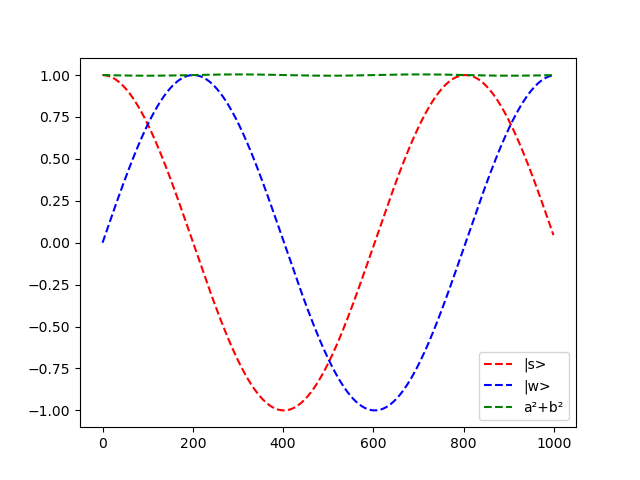
\includegraphics[scale=0.3]{Grover/grover_n16_1000.png}
  \caption{Evolution des amplitudes pour n=16, sur 1000 itérations}
  \label{fig:groverGraph}
\end{figure}

En bleu, on représente le module de l'état cible, en rouge le module des autres états (en vert, pour indication, la somme des modules au carré pour vérifier l'unitarité de l'état). On voit bien ici le rebouclement après $\frac{\pi}{4}\sqrt{N}$ itérations.

\section{Algorithme de Shor}

On peut enfin étudier l'algorithme de Shor, proposé par Peter Shor en 1997 \cite{Shor97}.

\begin{pb}
  On s'intéresse au problème de la factorisation d'un nombre $N=q \times q$ avec $p$ et $q$ nombres premiers très grands.
\end{pb}

Classiquement, ce problème est résolvable en $\mathcal{O}(\exp{[c . n^{\frac{1}{3}} (\log n)^{\frac{2}{3}} ]})$, par exemple avec l'algorithme du crible du corps algébrique \cite{NFS-RSA220}. Cet algorithme est certes efficace pour des nombres supérieurs à $10^{100}$, mais ne permet pas de factoriser pour des nombres de $2048$ ou $4096$ bits. Ce domaine de recherche avance rapidement, et de nouveaux algorithmes sont trouvés permettant d'améliorer les performances. On ne trouve en revanche toujours pas d'algorithmes permettant de résoudre ce problème en un temps polynomial.

En utilisant l'informatique quantique, Shor a démontré que ce problème était résolvable bien plus rapidement qu'en utilisant l'informatique classique, en un peu plus rapidement que $\mathcal{O}(n^3)$. En fait, Shor résout avec son algorithme une sous-partie de l'algorithme de la figure \ref{fig:algoshor}

\pagebreak
\begin{figure}[h]
  

\begin{algorithm}[H]
  \SetAlgoLined
  \KwData{N}
  \Repeat{}{
    choose a coprime with N;

    find smallest r such that $a^r \equiv 1 (mod N)$;

    \eIf{r is even}
    {
      $x \equiv a^{\frac{r}{2}} (mod N) $;

      \eIf{$x + 1 \not \equiv 0 (mod N)$}
      {
        at least one of $\{p, q\} \in \{gcd(x+1, N), gcd(x-1, N)\}$;

        break;
      }
      {
        continue;
      }
    }
    {
      continue;
    }
  }
\end{algorithm}
\caption{Algorithme de factorisation en nombres premiers}
\label{fig:algoshor}
\end{figure}


Cet algorithme permet de trouver les facteurs premiers $p$ et $q$. On peut prouver que la deuxième instruction revient à chercher la période de la fonction $a^r \Mod{N}$. C'est cette instruction spécifique qui est compliquée à résoudre classiquement, mais que Shor à réussi à résoudre en quantique.

Cet algorithme se passe en 3 étapes. Les deux premières sont similaires aux deux algorithmes précédents: on fait passer un n-qubit de l'état $\ket{0}^{\otimes n}$ à l'état équilibré; puis on évalue la fonction $a^r \Mod{N}$ pour l'état équilibré. La troisième étape fait intervenir une nouvelle notion: la transformée de Fourier quantique. C'est une généralisation de la porte de Hadamard, qui fait passer les qubits de la base $\{\ket{0}, \ket{1}\}$ à la base $\{\ket{+}, \ket{-}\}$ (pour rappel, on a $\ket{+} = \frac{1}{\sqrt{2}}(\ket{0} + \ket{1})$, et $\ket{-} = \frac{1}{\sqrt{2}}(\ket{0} - \ket{1})$).

La transformée de Fourier quantique peut être comprise ici en faisant l'analogie à la version classique. Dans un cas classique, quand on a une fonction périodique, l'application de la transformée de Fourier permet de passer de la représentation temporelle à la représentation fréquentielle. Sur cette représentation, on obtient des raies de Dirac aux fréquences correspondant aux périodes de la fonction. Il suffit alors de lire les valeurs pour obtenir les périodes. Il s'agit du même principe en quantique: la transformée de Fourier quantique nous permet d'obtenir directement la valeur de la période, avec l'avantage de faire le calcul parallélisé.

\medbreak

Cet algorithme a déjà été implémenté sur de réels processeurs quantique, permettant de factoriser 15 en 5 et 3 en 2001 \cite{Vandersypen01}, puis de factoriser 21 en 3 et 7 en 2011 \cite{Martin11}. Aucun travail expérimental n'a réussi à ce jour à factoriser des nombres plus grands que ça, limitant les risques potentiels à la cybersécurité engendrés par cet algorithme. La structure de la solution de Shor necessite en effet beaucoup de corrections d'erreur sur les mises en oeuvres pratiques dûes au bruits sur les grand nombres de portes utilisées, ce qui complexifie et ralentis les implémentations.

En revanche, ce problème de factorisation n'a pas pour seule solution celle proposée par Shor, et notamment une implémentations théorique de 2018 montre une factorisation d'entiers de 2048 bits en 8 heures, en utilisant 20 million de qubits \cite{gidney2019factor}. D'autres algorithmes sont présentés depuis 2010 notamment, présentant d'autres alternatives à Shor \cite{anschuetz2018variational}.
\input{includes/chap-05-perpectives.tex}
\chapter{Conclusion}

Ce travail bibliographique met en place les différents éléments necessaires à la compréhension de l'informatique quantique: la notion de système quantique, et la restriction aux qubits, les mécanismes permettant de faire évoluer les systèmes, ainsi que la mesure. On illustre de plus trois algorithmes majeurs dans l'histoire de ce domaine, en montrant leur champs d'application, les problèmes qu'ils permettent de résoudre. De tout ce travail découle la conclusion que l'informatique quantique permet d'accélérer considérablement la résolution d'un certain nombre de problèmes irrésolvables avec les technologies classiques.

En revanche, un certain nombre de problèmes restent ouverts à la suite de ce travail:

\begin{itemize}
    \item Sur la construction effective des circuits, est-il optimal de décomposer le circuit en portes élémentaires CNOT ou est-il plus rapide de juste exécuter le problème classiquement ? La question se pose en particulier pour l'algorithme de Deutsch-Jozsa où l'oracle a besoin, a priori, d'être construit en connaissant déjà toutes les sorties de la fonction.
    \item Sur l'algorithme de Deutsch-Jozsa encore une fois, que se passe-t-il quand on l'applique à d'autres classes de fonction, et comment peut-on l'adapter pour différencier d'autres types de fonctions ?
    \item Sur le problème de Deutsch-Jozsa, peut-on trouver un autre algorithme permettant de résoudre le problème ? Cela amène vers l'écriture des contraintes algébriques necessaires à la résolution du problème, et d'essayer de déterminer si la solution proposée par Deutsch-Jozsa est optimale ou non.
    \item En étendant le point précédent, peut-on poser des contraintes algébriques sur les problèmes ou écrire des spécifications algébriques pour les différents algorithmes ? Cela permettrait de caractériser systématiquement les problèmes pouvant disposer d'une amélioration quantique.
\end{itemize}

\begin{appendix}
\chapter{Algorithme de Deutsch-Jozsa}

\section{Problème à résoudre}

Pour rappel, on cherche à déterminer si une fonction $f$ booléenne définie par

\[
  \begin{array}{llll}
    f :  &  \{0, 1\}^n              & \to       & \{ 0, 1 \} \\
         &  (x_0, x_1, \dots , x_n) & \mapsto   &  y = f(x_0, x_1, \dots , x_n), 
  \end{array}  
\]

est équilibrée ou constante. On sait à l'avance que $f$ est soit constante, soit équilibrée, mais ne peut pas être aucun.

% \begin{definition}
%   Une fonction booléenne $f$ est dite équilibrée si $f$ retourne 0
%   pour la moitié de ses entrées.
% \end{definition}

% \begin{definition}
%   Une fonction est dite constante si elle retourne une constante pour
%   toutes ses entrées.
% \end{definition}


% \begin{rem}
%   Avec $n$ un entier et comme les fonctions booléennes sont à valeur
%   dans $\{0,1\}$, il n'existe que deux fonctions constantes $f_0$ et
%   $f_1$.
% \end{rem}

\begin{ex}
  Soit $f$ la fonction booléenne $f : \{0,1\}^2 \to \{0,1\}$ définie
  par la table de vérité suivante :
\[
  \begin{array}{|c|c|}
    \hline
   (x_1, x_2) & f(x_1,x_2) \\
    \hline
    (0,0) & 0 \\
    \hline
    (0,1) & 1 \\
    \hline
    (1,0) & 1 \\
    \hline
    (1,1) & 0 \\
    \hline
  \end{array}
\]
Cette fonction est équilibrée. On notera qu'elle correspond au
classique ``ou exclusif''. Cette fonction pourrait être représentée
par le vecteur de ces valeurs : $(0,1,1,0)$. Elle peut aussi être
codée en listant les entrées où elle est vraie, ici $\{(0,1),(1,0)\}$ (ou bien en base 10: $\{1, 2\}$).
\end{ex}

\subsubsection{Initialisation}
On commence avec :
$\ket{u_0} = (\ket{0}^{\bigotimes n}) \otimes \ket{1}$
: n-qubits à $\ket{0}$ et 1-qubit à $\ket{1}$.

%% PASSER CA EN ANNEXES
\subsubsection{Etape 1}

On applique une porte de Hadamard à $\ket{u_0}$ pour avoir un état équiprobable:
$\ket{u_1} = H\ket{u_0} = \frac{1}{\sqrt{2^{n + 1}}}
\displaystyle\sum_{x=0}^{2^n-1} \ket{x}(\ket{0} - \ket{1})$.

\subsubsection{Etape 2}
On applique l'oracle quantique suivant à $\ket{u_1}$:
\[ o : \ket{x}\ket{y}\mapsto \ket{x}\ket{y\oplus f(x)}. \]

Posons $x$, on est alors dans l'une des deux situations disjointes suivantes :
\begin{itemize}
\item $f(x) = 0$,
\item $f(x) = 1$.
\end{itemize}

Analysons chacune de ces situations, tout d'abord si $f(x) = 0$ alors
%Prenons le cas à 1 qubit:
\[
o : \ket{x}(\ket{0} - \ket{1}) \mapsto \ket{x}(\ket{0} - \ket{1}).
\]
Autrement dit $\ket{x}(\ket{0} - \ket{1}$ est un  point fixe de $o$.

Dans l'autre situation, on a $f(x) = 1$ et on en déduit
\[
o : \ket{x}(\ket{0} - \ket{1}) \mapsto \ket{x}(\ket{1} - \ket{0}).
\]
Autrement dit, dans ce cas, le vecteur $\ket{x}(\ket{0} - \ket{1})$
est envoyé sur son opposé via $o$.

Finalement, les deux cas précédents peuvent être résumé sous la forme suivante
\[
o : \ket{x}(\ket{0} - \ket{1}) \mapsto (-1)^{f(x)}\ket{x}(\ket{0} - \ket{1}).
\]

Par linéarité, on en déduit :

\begin{equation}\ket{u_2} = \frac{1}{\sqrt{2^{n + 1}}} 
\displaystyle\sum_{x=0}^{2^n-1} (-1)^{f(x)}\ket{x}(\ket{0} - \ket{1}) .
\end{equation}

On peut ignorer le dernier qubit ($\ket{0} - \ket{1}$) comme il est
constant. Finalement, on en déduit :
\begin{equation}
\ket{u_2} = \frac{1}{\sqrt{2^{n + 1}}}
\displaystyle\sum_{x=0}^{2^n-1} (-1)^{f(x)}\ket{x}.
\end{equation}

\subsubsection{Etape 3}

% Maintenant qu'on a appliqué notre oracle, on est toujours dans un état
% "probabiliste", et en mesurant nous n'obtiendrons pas une réponse
% exacte à notre problème. L'objectif est donc maintenant de ramener les
% solutions sur un état déterminé pour obtenir la réponse
% systématique. En appliquant la porte de Hadamard, on va pouvoir forcer
% un état à apparaître pour un type de fonction $f$, et le forcer à
% disparaître dans l'autre cas, ce qui nous permet d'avoir une réponse
% systématique sur le type de la fonction : est-elle équilibrée ou bien constante ?

On réapplique une porte Hadamard à chaque qubit sortant, ce qui donne:

\[ 
  \ket{u_3} = \frac{1}{\sqrt{2^{n}}}
\displaystyle\sum_{x=0}^{2^n-1} (-1)^{f(x)} \left( \frac{1}{\sqrt{2^{n}}} \displaystyle\sum_{y=0}^{2^n-1} (-1)^{x.y}\ket{y} \right) .
\]

Par linéarité, on a :
\begin{equation}
  \label{eq:1}
  \ket{u_3} = \frac{1}{2^{n}}
  \displaystyle\sum_{x=0}^{2^n-1} \displaystyle\sum_{y=0}^{2^n-1}(-1)^{f(x)} (-1)^{x.y}\ket{y}  .
\end{equation}

La probabilité $|p|$ de mesurer $\ket{0}^{\bigotimes n}$ est donc : 
\begin{equation}
  \label{eq:2}
  |\frac{1}{2^{n}}\displaystyle\sum_{x=0}^{2^n-1}(-1)^{f(x)}|,
\end{equation}

avec $p = \frac{1}{2^{n}}\displaystyle\sum_{x=0}^{2^n-1}(-1)^{f(x)}$.

Si on a une fonction $f(x)$ constante, alors chaque élément de la
somme retourne la même valeur (1 ou -1 suivant que $f(x)$ retourne 0
ou 1), la somme va donc valoir $\pm 2^{n}$. Dans le cas où la fonction
est équilibrée, on va avoir autant de 1 que de -1, la somme est donc
nulle.

On a donc les valeurs suivantes dépendant du type de $f(x)$ :
\begin{enumerate}
  \item Si $f(x)$ est constante :  $p = \pm \frac{1}{2^n} \times 2^{n} = \pm 1$,
  \item Si $f(x)$ est équilibrée : $p = \pm \frac{1}{2^n} \times 0 = 0$.
\end{enumerate}

Dans le cas constant, on ne peut donc que mesurer $\ket{0}^{\bigotimes n}$ puisqu'il a une probabilité de 1 d'apparaître. Dans le cas équilibré, on ne mesure jamais $\ket{0}^{\bigotimes n}$ puisque sa probabilité est nulle.

On en conclue que, lorsqu'on effectue une mesure, si on tombe sur $\ket{0}^{\bigotimes n}$ alors la fonction est constante, sinon elle est équilibrée.

%'objectif de cette dernière étape est de passer 

\subsection{Exemple}

Prenons une fonction $f$ comme définie précédemment avec $n=2$, sans
savoir si elle est constante ou équilibrée.

\subsubsection{Etape 1}


On commence avec $\ket{u_0} = \ket{001}$. La première étape est
l'application de la porte d'hadamard à $\ket{u_0}$:

\begin{align}
\ket{u_1} &= H\ket{u_0} = H\ket{0} \otimes H\ket{0} \otimes H\ket{1} \nonumber ,\\
& = \frac{1}{2\sqrt{2}} \left( (\ket{0} + \ket{1})\otimes(\ket{0} + \ket{1})\otimes(\ket{0} - \ket{1}) \right) \nonumber ,\\
 & = \frac{1}{2\sqrt{2}}\{\ket{000} - \ket{001} + \ket{010} - \ket{011} + \ket{100} - \ket{101} + \ket{110} - \ket{111}\} \nonumber ,\\
& = \frac{1}{2\sqrt{2}}\{\ket{00}(\ket{0} - \ket{1}) + \ket{01}(\ket{0} - \ket{1}) + \ket{10}(\ket{0} - \ket{1}) + \ket{11}(\ket{0} - \ket{1})\} .
\end{align}

%On peut factoriser le tout par $(\ket{0} - \ket{1})$: 
%$

\subsubsection{Etape 2: oracle quantique}

On applique à $\ket{u_1}$ l'oracle quantique $\ket{x}\ket{y}\rightarrow\ket{x}\ket{y\oplus f(x)}:$

\begin{align*}
\ket{u_2}  =  \frac{1}{2\sqrt{2}}  & \ket{00}(\ket{0 \oplus f(00)} - \ket{1 \oplus f(00)}) + \\
& \ket{01}(\ket{0 \oplus f(01)} - \ket{1 \oplus f(01)}) + \\
& \ket{10}(\ket{0 \oplus f(10)} - \ket{1 \oplus f(10)}) + \\
& \ket{11}(\ket{0 \oplus f(11)} - \ket{1 \oplus f(11)}).
\end{align*}


On peut alors réécrire l'équation de la façon suivante: 



\begin{align*}
  \ket{u_2} = \frac{1}{2\sqrt{2}} & (-1)^{f(00)} \ket{00}  (\ket{0} - \ket{1}) + \\
&(-1)^{f(01)} \ket{01}  (\ket{0} - \ket{1}) + \\
&(-1)^{f(10)} \ket{10}  (\ket{0} - \ket{1}) + \\
&(-1)^{f(11)} \ket{11}  (\ket{0} - \ket{1}) .
\end{align*}

Par la suite, on va appliquer une porte de Hadamard à $\ket{u_2}$. Le qubit $\ket{0} - \ket{1}$ donne $\ket{1}$ par la cette porte, il est donc constant par rapport à $\ket{u_0}$. On peut donc le retirer de l'équation, ce qui nous donne pour $\ket{u_2}$ :

\begin{equation}
  \label{eq:3}
\ket{u_2} = \frac{1}{2\sqrt{2}} \left( (-1)^{f(00)} \ket{00} + (-1)^{f(01)} \ket{01} + (-1)^{f(10)} \ket{10} + (-1)^{f(11)} \ket{11} \right). 
\end{equation}


Matriciellement, on peut donc écrire

\begin{equation}
  \label{eq:4}
\ket{u_2} = \left(  \begin{array}{cccc}
     (-1)^{f(00)}  &0 & 0 &0 \\
     0 & (-1)^{f(01)} & 0 &0 \\
     0 &0 & (-1)^{f(10)} &0 \\
     0 &0 & 0 & (-1)^{f(11)} \\
        \end{array}
      \right)
      \left(  \begin{array}{c}
                1 \\
                1 \\
                1 \\
                1 
              \end{array}
      \right).
\end{equation}


\subsubsection{Etape 3: porte de Hadamard}

On applique donc une porte de hadamard à $\ket{u_2}$:
\begin{equation}
  \label{eq:5}
\ket{u_3} = \frac{1}{2\sqrt{2}} H \left( (-1)^{f(00)} \ket{00} + (-1)^{f(01)} \ket{01} + (-1)^{f(10)} \ket{10} + (-1)^{f(11)} \ket{11} \right) .
\end{equation}

Nous sommes sur une porte de hadamard pour 2 qubits, ce qui donne
la relation matricielle suivante pour $\ket{u_3}$:

\begin{align}
\ket{u_3} &=
\frac{1}{4} 
\begin{bmatrix}
  1 & 1 & 1 & 1 \\
  1 & -1 & 1 & -1 \\
  1 & 1 & -1 & -1 \\
  1 & -1 & -1 & 1 \\
\end{bmatrix}
\begin{bmatrix}
  (-1)^{f(00)} \\ (-1)^{f(01)} \\ (-1)^{f(10)} \\ (-1)^{f(11)}
\end{bmatrix} , \nonumber \\ 
 &= \frac{1}{4} 
\begin{bmatrix}
  (-1)^{f(00)} + (-1)^{f(01)} + (-1)^{f(10)} + (-1)^{f(11)} \\
  (-1)^{f(00)} - (-1)^{f(01)} + (-1)^{f(10)} - (-1)^{f(11)} \\
  (-1)^{f(00)} + (-1)^{f(01)} - (-1)^{f(10)} - (-1)^{f(11)} \\
  (-1)^{f(00)} - (-1)^{f(01)} - (-1)^{f(10)} + (-1)^{f(11)} \\
\end{bmatrix}.
\end{align}

Si f est constante , alors
$(-1)^{f(00)} = (-1)^{f(01)} = (-1)^{f(10)} = (-1)^{f(11)}$. En
fonction du fait que $f=0$ ou bien $f=1$:

\begin{equation}
  \label{eq:6}
\ket{u_3}=
\begin{bmatrix}
  1 \\ 0 \\ 0 \\ 0
\end{bmatrix}  \text{ ou bien }
\ket{u_3}=
\begin{bmatrix}
  -1 \\ 0 \\ 0 \\ 0
\end{bmatrix}.
\end{equation}
On a donc une probabilité de $1$ de mesurer l'état $\ket{00}$.

En revanche, si f est équilibrée, la moitié des valeurs vont
valoir $(-1)^{0} = 1$ et l'autre moitié $(-1)^{1} = -1$. La première
ligne du vecteur $\ket{u_3}$ donne donc systématiquement 0, on ne mesure donc
jamais l'état $\ket{00}$.

\pagebreak

\section{Visualisation géométrique}
Reprenons cet algorithme avec $n=4$ qubits et affichons l'évolution des états des qubits avec des sphères de bloch.

\subsection{Fonction constante $f_0(x)$ = 0}

\begin{figure}[ht]
  \centering
  \begin{subfigure}{0.8\textwidth}
    \centering
    \begin{subfigure}[b]{0.6\textwidth}
      \centering
      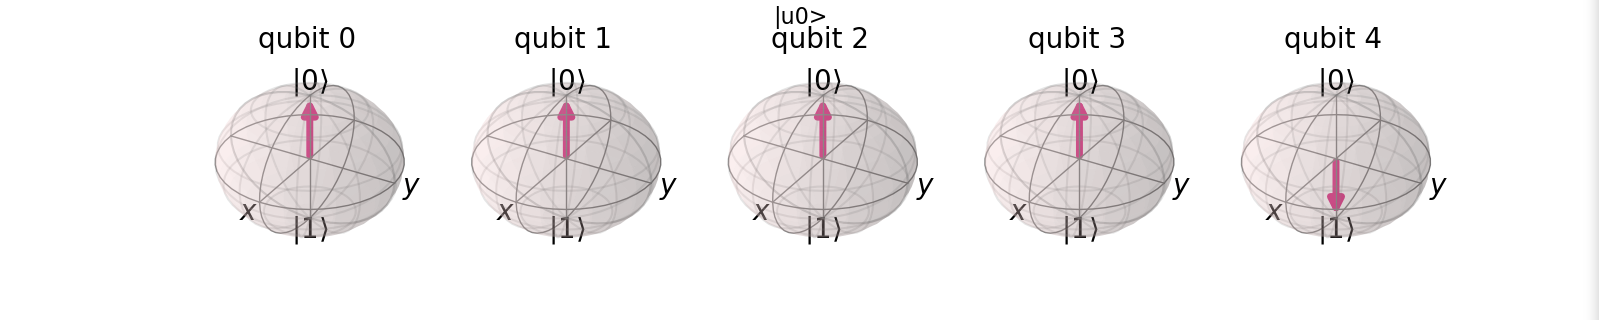
\includegraphics[width=\textwidth]{DJ/visualization_constant_1_u0.png}
    \end{subfigure}
    \begin{subfigure}[b]{0.25\textwidth}
      \centering
      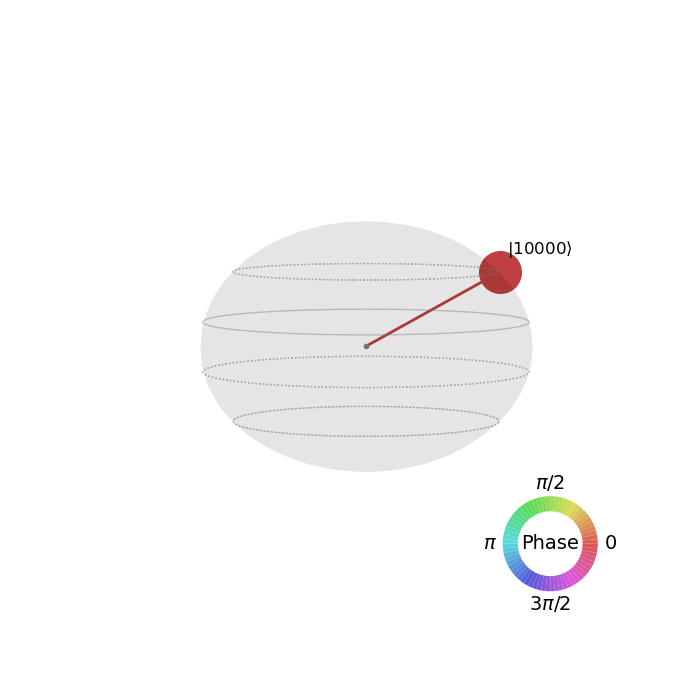
\includegraphics[width=\textwidth]{DJ/visualization_constant_2_u0.png}
    \end{subfigure}
    \caption{$\ket{u0}=\ket{00001}$}
  \end{subfigure}

  \begin{subfigure}{0.8\textwidth}
    \centering
    \begin{subfigure}[b]{0.6\textwidth}
      \centering
      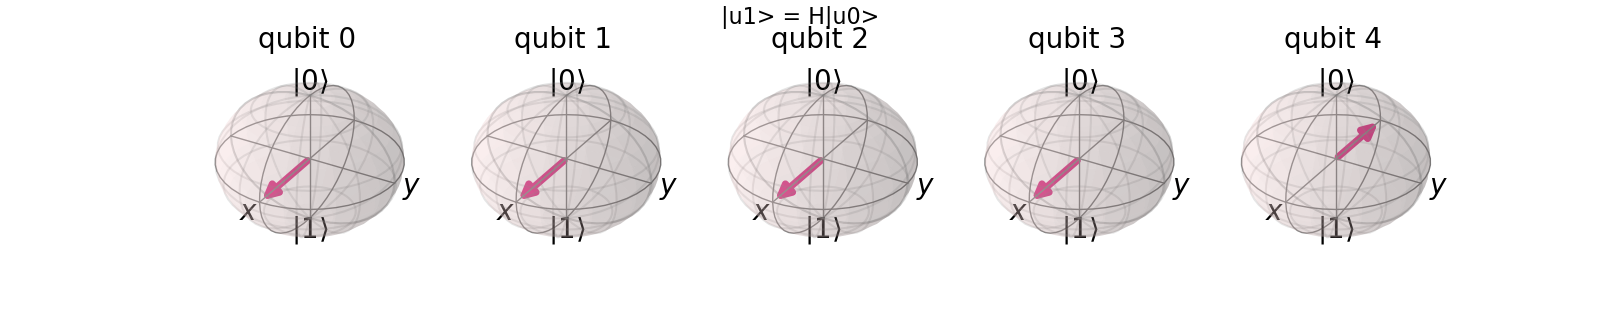
\includegraphics[width=\textwidth]{DJ/visualization_constant_1_u1.png}
    \end{subfigure}
    \begin{subfigure}[b]{0.25\textwidth}
      \centering
      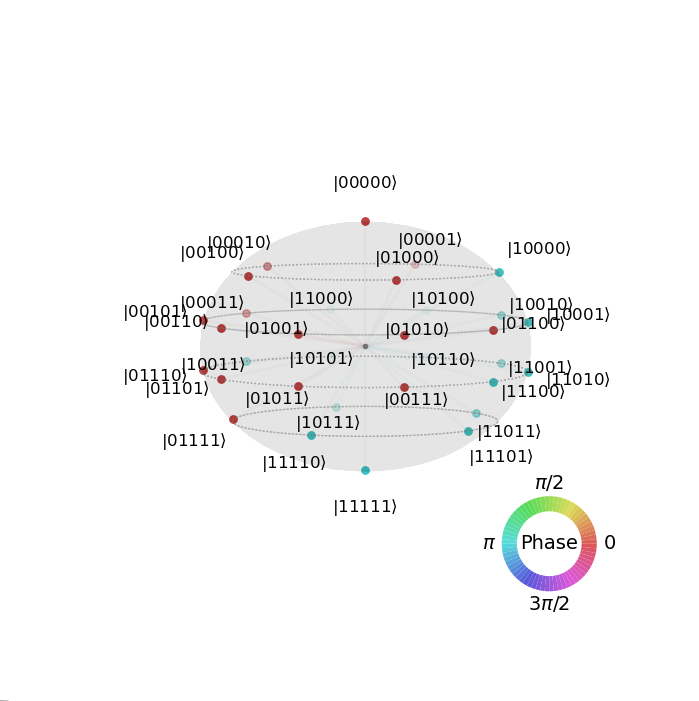
\includegraphics[width=\textwidth]{DJ/visualization_constant_2_u1.png}
    \end{subfigure}
    \caption{$\ket{u1}=H\ket{u0} = \ket{++++-}$}
  \end{subfigure}

  \begin{subfigure}{0.8\textwidth}
    \centering
    \begin{subfigure}[b]{0.6\textwidth}
      \centering
      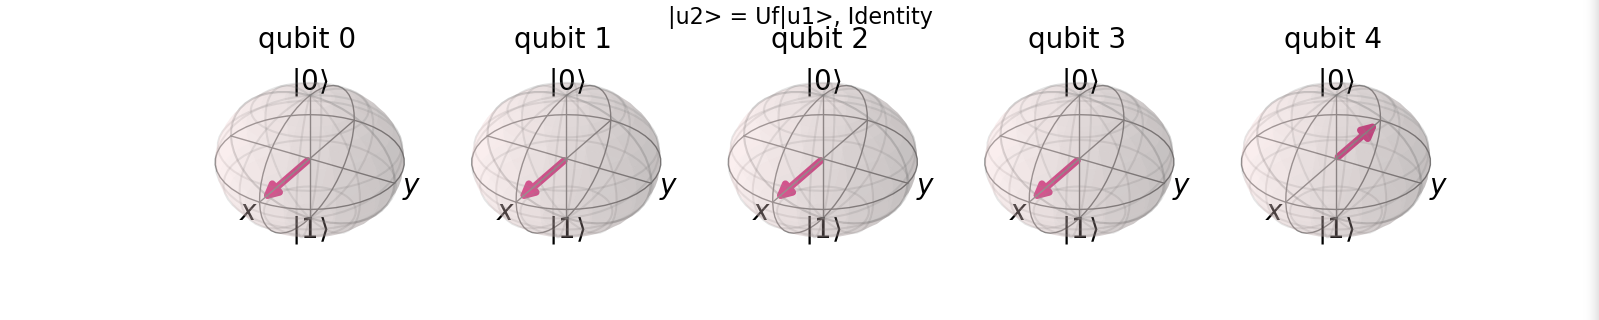
\includegraphics[width=\textwidth]{DJ/visualization_constant_1_u2.png}
    \end{subfigure}
    \begin{subfigure}[b]{0.25\textwidth}
      \centering
      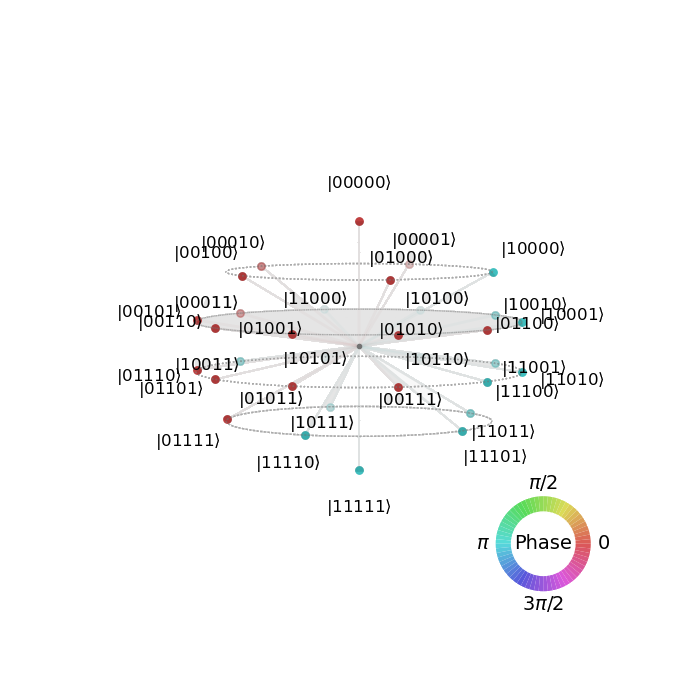
\includegraphics[width=\textwidth]{DJ/visualization_constant_2_u2.png}
    \end{subfigure}
    \caption{$\ket{u2}=U_f\ket{u1} = \ket{++++-}$}
  \end{subfigure}

  \begin{subfigure}{0.8\textwidth}
    \centering
    \begin{subfigure}[b]{0.6\textwidth}
      \centering
      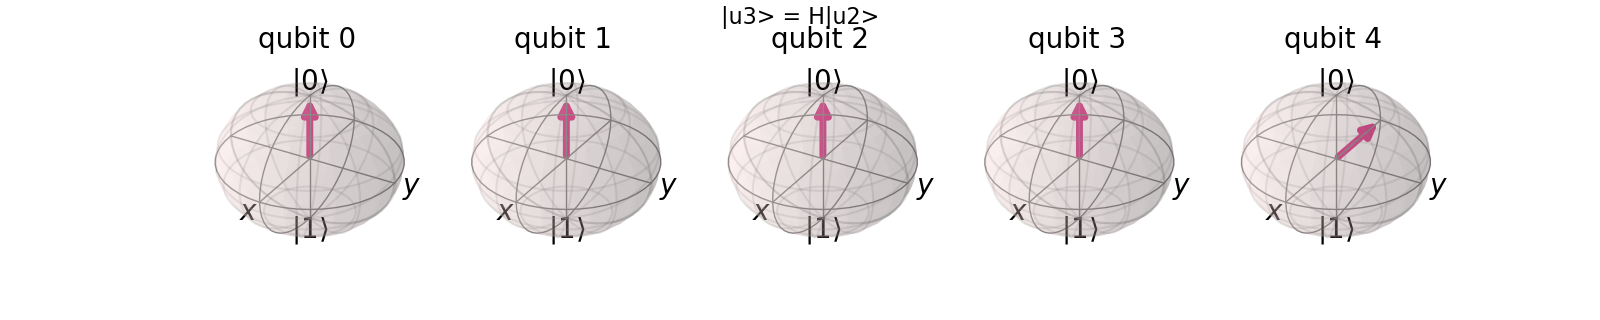
\includegraphics[width=\textwidth]{DJ/visualization_constant_1_u3.png}
    \end{subfigure}
    \begin{subfigure}[b]{0.25\textwidth}
      \centering
      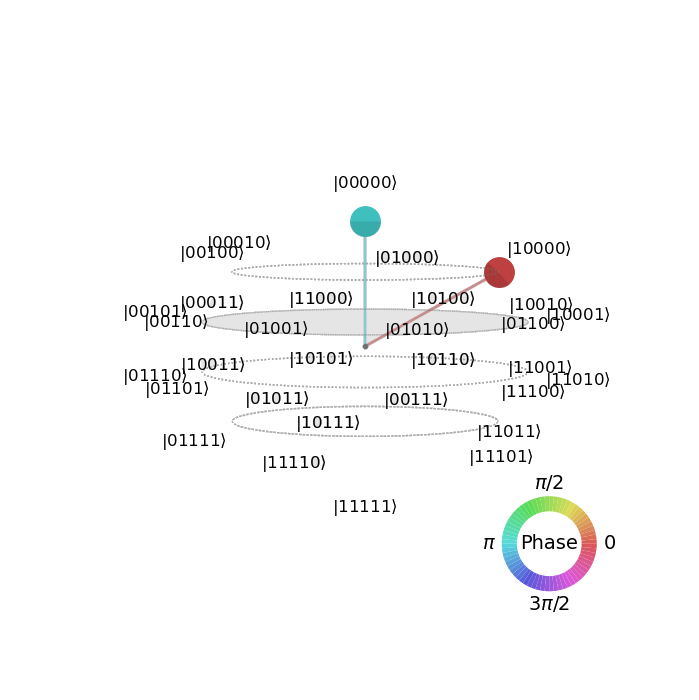
\includegraphics[width=\textwidth]{DJ/visualization_constant_2_u3.png}
    \end{subfigure}
    \caption{$\ket{u3}=H\ket{u2}= \ket{0000}\ket{-}$}
  \end{subfigure}

  \caption{Evolution des états pour une fonction f constante, vecteurs d'états séparés et réunis}
\end{figure}

On voit ici l'ensemble des états que prends le registre de sortie. Dans le cas constant, on se retrouve bien à mesure exclusivement la valeur 0 (pour rappel, on ne mesure pas le dernier qubit qui est constant à 1). Pour les deux étapes intermédiaires, on visualise bien qu'on se retrouve dans une certaine superposition des états possibles. A noter, la visualisation présentée dans la colonne de gauche montre les états séparés. On peut rappeler que cette représentation n'est possible que parce que le 4-qubit est dans un état séparable. La représentation serait impossible si il était dans un état superposé (par exemple, si $\ket{u} = \frac{1}{2}(\ket{10001} + \ket{01001})$).

\subsection{Fonction équilibrée quelconque $f_1(x)$}
La figure suivante présente la même visualisation, pour une fonction équilibrée:

\begin{figure}[ht]
  \centering
  \begin{subfigure}{0.65\textwidth}
    \centering
    \begin{subfigure}[b]{0.6\textwidth}
      \centering
      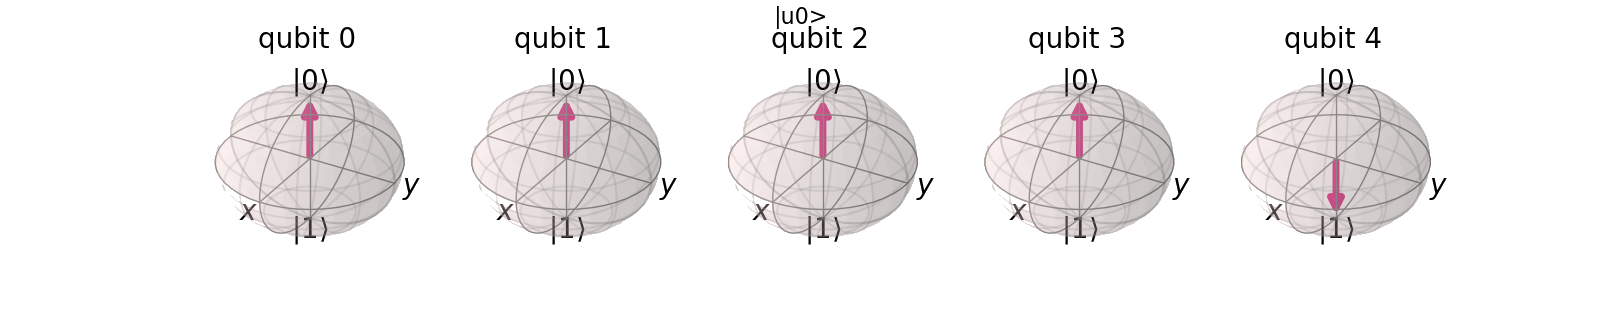
\includegraphics[width=\textwidth]{DJ/visualization_eq_1_u0.png}
    \end{subfigure}
    \begin{subfigure}[b]{0.23\textwidth}
      \centering
      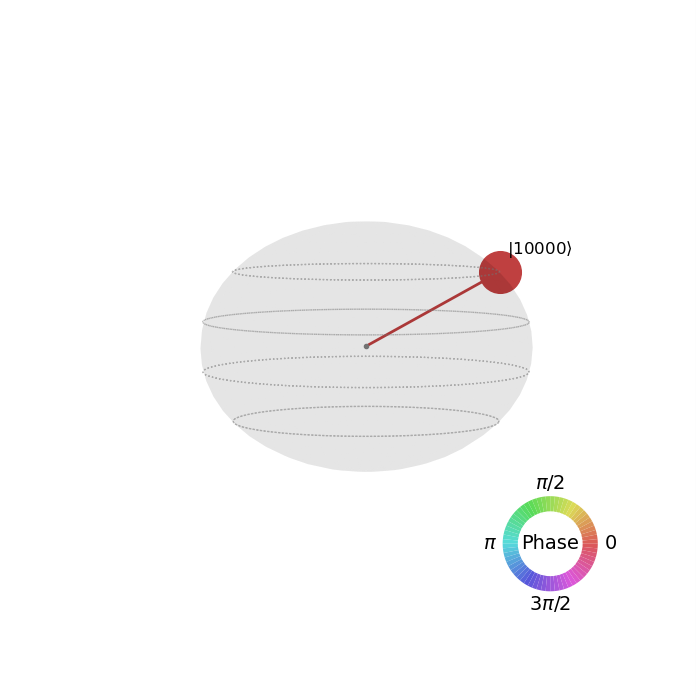
\includegraphics[width=\textwidth]{DJ/visualization_eq_2_u1.png}
    \end{subfigure}
    \caption{$\ket{u0}=\ket{0001}$}
  \end{subfigure}

  \begin{subfigure}{0.65\textwidth}
    \centering
    \begin{subfigure}[b]{0.6\textwidth}
      \centering
      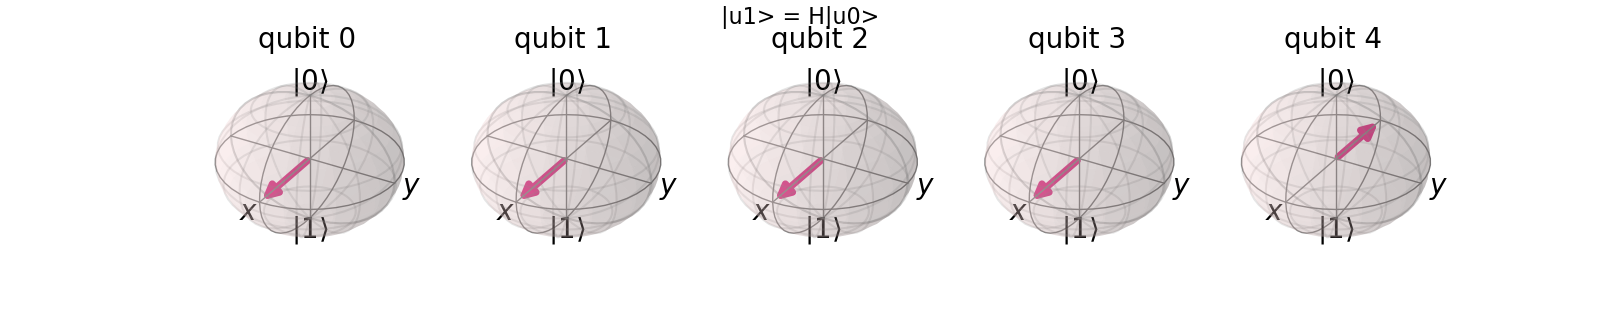
\includegraphics[width=\textwidth]{DJ/visualization_eq_1_u1.png}
    \end{subfigure}
    \begin{subfigure}[b]{0.23\textwidth}
      \centering
      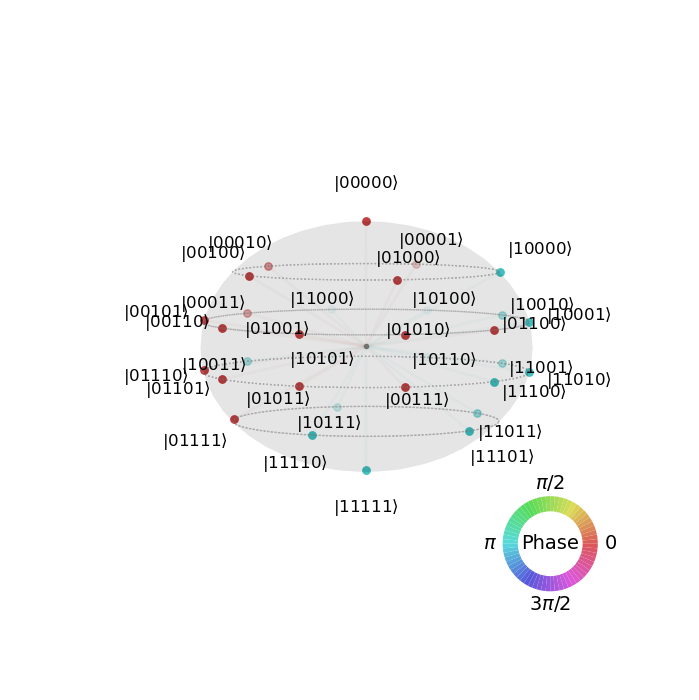
\includegraphics[width=\textwidth]{DJ/visualization_eq_2_u2.png}
    \end{subfigure}
    \caption{$\ket{u1} = H\ket{u0} = \ket{++++-}$}
  \end{subfigure}

  \begin{subfigure}{0.65\textwidth}
    \centering
    \begin{subfigure}[b]{0.6\textwidth}
      \centering
      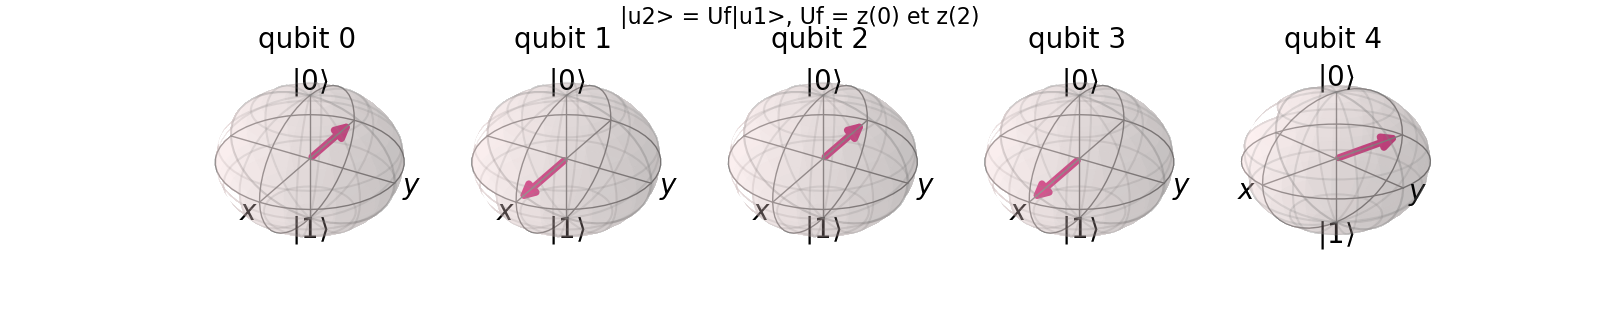
\includegraphics[width=\textwidth]{DJ/visualization_eq_1_u2.png}
    \end{subfigure}
    \begin{subfigure}[b]{0.23\textwidth}
      \centering
      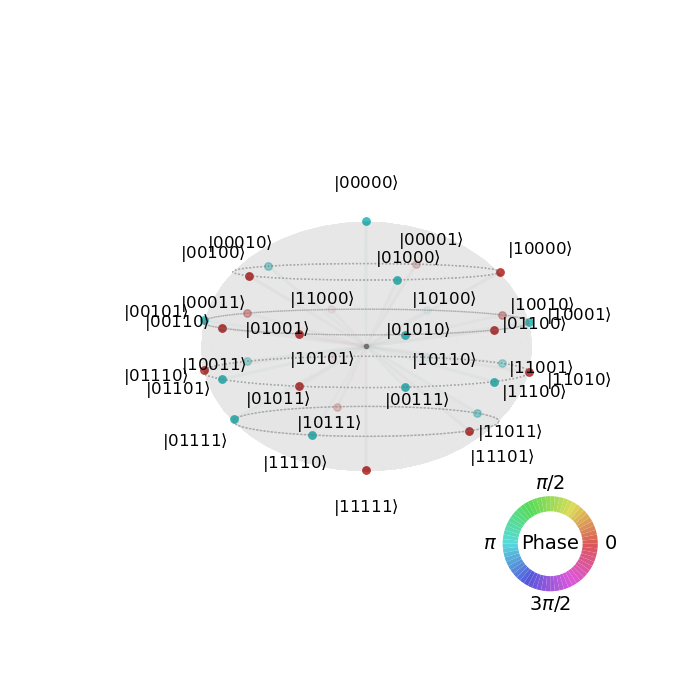
\includegraphics[width=\textwidth]{DJ/visualization_eq_2_u3.png}
    \end{subfigure}
    \caption{$\ket{u2} = U_f\ket{u1} = \ket{-+-+-}$}
  \end{subfigure}

  \begin{subfigure}{0.65\textwidth}
    \centering
    \begin{subfigure}[b]{0.6\textwidth}
      \centering
      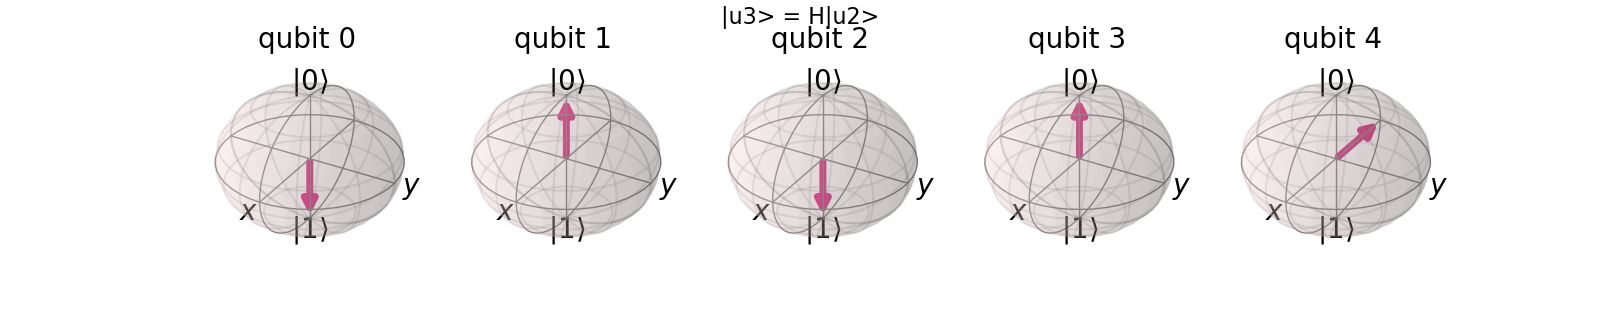
\includegraphics[width=\textwidth]{DJ/visualization_eq_1_u3.png}
    \end{subfigure}
    \begin{subfigure}[b]{0.23\textwidth}
      \centering
      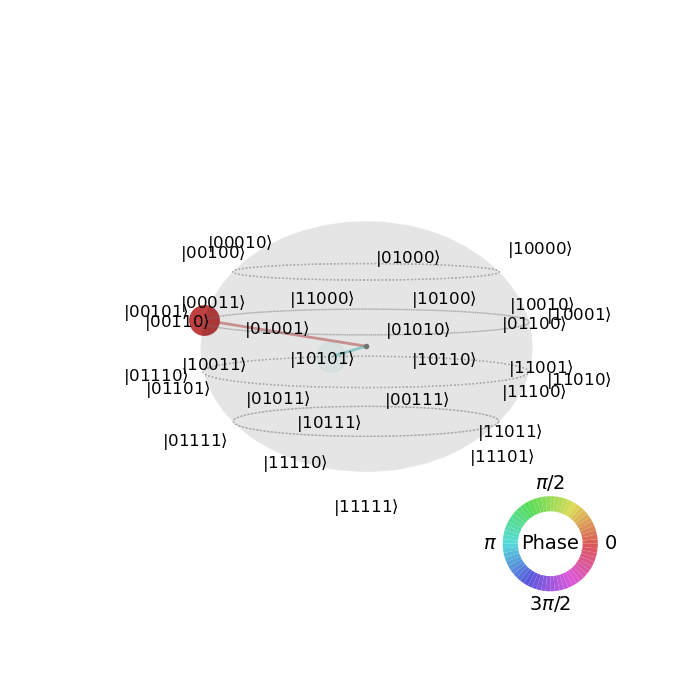
\includegraphics[width=\textwidth]{DJ/visualization_eq_2_u4.png}
    \end{subfigure}
    \caption{$\ket{u3}=H\ket{u2} = \ket{1010}\ket{-}$}
  \end{subfigure}
  \caption{Evolution des états pour une fonction f équilibrée, vecteurs d'états séparés}
\end{figure}

% \begin{tikzpicture}
%   % Define radius
%   \def\r{2}
%   % Bloch vector
%   \draw (0,0) node[circle,fill,inner sep=1] (orig) {} -- (\r/3,\r/2) node[circle,fill,inner sep=0.7,label=above:$\vec{a}$] (a) {};
%   \draw[dashed] (orig) -- (\r/3,-\r/5) node (phi) {} -- (a);

%   % Sphere
%   \draw (orig) circle (\r);
%   \draw[dashed] (orig) ellipse (\r{} and \r/3);

%   % Axes
%   \draw[->] (orig) -- ++(-\r/5,-\r/3) node[below] (x1) {$X$};
%   \draw[->] (orig) -- ++(\r,0) node[right] (x2) {$Y$};
%   \draw[->] (orig) -- ++(0,\r) node[above] (x3) {$\ket{0}$};

%   % %Angles
%   % \pic [draw=gray,text=gray,->,"$\phi$"] {angle = x1--orig--phi};
%   % \pic [draw=gray,text=gray,<-,"$\theta$"] {angle = a--orig--x3};

% \end{tikzpicture}

\medbreak

On voit bien sur cette figure que dans le cas d'une fonction équilibrée, l'état va se situer à un des points indiqués sur la sphère de Bloch mais jamais sur le point 0. 

\chapter{Algorithme de Bernstein-Vazirani}
\section{Problème à résoudre}

Soient $x$ et $s$ tels que $x, s \in \{0, 1\}^n$.

On pose une fonction $f$ définie par:
\[
  \begin{array}{llll}
    f :  &  x              & \to     & y = s \cdot x \Mod{2} = x_1 s_1 + x_2 s_2 + \dots + x_n s_n \\
    f:   &  \{0, 1\}^n     & \to     & \{0, 1\},
  \end{array}  
\]

\begin{ex}
  Soit $s$ le mot booléen suivant: $s = 10$. La fonction $f$ a donc la table de vérité suivante:
\[
  \begin{array}{|c|c|c|}
    \hline
   (x_1, x_2) & s & f(x_1,x_2) \\
    \hline
    (0,0) & 10 & 0 \\
    \hline
    (0,1) & 10 & 0 \\
    \hline
    (1,0) & 10 & 1 \\
    \hline
    (1,1) & 10 & 1 \\
    \hline
  \end{array}
\]
On observe que le résultat est de 1 pour les entrées $(x_1, x_2)$ où l'emplacement des $1$ correspond à ceux de $s$.
\end{ex}

\begin{pb}[Bernstein-Vazirani]
Etant donné un mot $s$ secret, et la fonction $f$ implémentant l'opération décrite précédemment, comment peut on retrouver $s$ en le moins d'évaluations de $f$ possibles ?
\end{pb}

\subsection{Solution classique}
Dans le cas classique, on va devoir évaluer au pire toutes les valeurs possibles de $s$ pour trouver sa valeur, soit $n$ évaluations de $f$. C'est un algorithme de complexité $\mathcal{O}(n)$.

\subsection{Solution quantique}
Dans le cas quantique, ce problème se résout en une seule évaluation
quantique de $f$. L'algorithme reprend celui de Deutsch-Jozsa en changeant la fonction appliquée dans l'oracle quantique.

\subsubsection{Initialisation}
On commence avec :
$\ket{u_0} = (\ket{0}^{\bigotimes n})$
: n-qubits à $\ket{0}$.

\subsubsection{Etape 1}

On applique une porte de Hadamard à $\ket{u_0}$ pour avoir un état équiprobable:
$\ket{u_1} = H\ket{u_0} = \frac{1}{\sqrt{2^n}}
\displaystyle\sum_{x=0}^{2^n-1} \ket{x}$.

\subsubsection{Etape 2}
On applique l'oracle quantique suivant à $\ket{u_1}$:
\[ o : \ket{x}\ket{y}\mapsto \ket{x}\ket{y\oplus (s \cdot x \Mod{2})}. 
\]

En suivant exactement le même raisonnement que pour Deutsch-Jozsa, on arrive à l'expression suivante: 

\begin{equation}\ket{u_2} = \frac{1}{\sqrt{2^n}}
\displaystyle\sum_{x=0}^{2^n-1} (-1)^{s \cdot x \Mod{2}}\ket{x}.
\end{equation}

\subsubsection{Etape 3}

De la même façon à Deutsch-Jozsa, on applique une porte Hadamard à chaque qubit sortant, ce qui donne:

% \[ \ket{u_3} = \frac{1}{\sqrt{2^{n}}}
% \displaystyle\sum_{x=0}^{2^n-1} (-1)^{s \cdot x \Mod{2}} \left( \frac{1}{\sqrt{2^{n}}} \displaystyle\sum_{y=0}^{2^n-1} (-1)^{x.y}\ket{y} \right) \]

\begin{align}
  \ket{u_3} & = \frac{1}{\sqrt{2^{n}}}
  \displaystyle\sum_{x=0}^{2^n-1} (-1)^{s \cdot x \Mod{2}} \left( \frac{1}{\sqrt{2^{n}}} \displaystyle\sum_{y=0}^{2^n-1} (-1)^{x.y}\ket{y} \right) \nonumber ,\\
  &= \frac{1}{\sqrt{2^{n}}}\displaystyle\sum_{x=0}^{2^n-1} (-1)^{s \cdot x \Mod{2}} \left( \frac{1}{\sqrt{2^{n}}} \displaystyle\sum_{y=0}^{2^n-1} (-1)^{x.y}\ket{y} \right) \nonumber ,\\
  & = \frac{1}{2^{n}} \displaystyle\sum_{x=0}^{2^n-1} \displaystyle\sum_{y=0}^{2^n-1} (-1)^{(s \cdot x \Mod{2}) + x.y} \ket{y} .
  \end{align}

Et on peut prouver que $\frac{1}{2^{n}} \displaystyle\sum_{x=0}^{2^n-1} \displaystyle\sum_{y=0}^{2^n-1} (-1)^{(s \cdot x \Mod{2}) + x.y} \ket{y}$ est égal à $\ket{s}$.
% (\textit{à faire ...})

\subsection{Exemple}

Prenons par exemple $s=(10)_2 = 2_{10}$, soit $f(x) = 2 \cdot x \Mod{2}$.
\subsubsection*{Etape 1: porte de Hadamard}

On commence avec $\ket{u_0} = \ket{00}$. La première étape est
l'application de la porte d'Hadamard à $\ket{u_0}$:

\begin{align}
\ket{u_1} &= H\ket{u_0} = H\ket{0} \otimes H\ket{0} \nonumber ,\\
& = \frac{1}{2} \left( (\ket{0} + \ket{1})\otimes(\ket{0} + \ket{1}) \right) \nonumber ,\\
 & = \frac{1}{2}\{\ket{00} + \ket{01} + \ket{10} + \ket{11}\}
\end{align}

%On peut factoriser le tout par $(\ket{0} - \ket{1})$: 
%$

\subsubsection*{Etape 2: oracle quantique}

On applique à $\ket{u_1}$ l'oracle quantique $\ket{x}\ket{y}\rightarrow\ket{x}\ket{y\oplus (s \cdot x \Mod{2})} = :$

\begin{align}
  \ket{u_2} &= \frac{1}{2}((-1)^{10 \cdot 00 \Mod{2}} \ket{00} + (-1)^{10 \cdot 01 \Mod{2}} \ket{01} + (-1)^{10 \cdot 10 \Mod{2}} \ket{10} + (-1)^{10 \cdot 11 \Mod{2}} \ket{11}) \nonumber ,\\
  &= \frac{1}{2}((-1)^{0} \ket{00} + (-1)^{0} \ket{01} + (-1)^{1} \ket{10} + (-1)^{1} \ket{11}) \nonumber ,\\
  &= \frac{1}{2} (\ket{00} + \ket{01} - \ket{10} - \ket{11})
\end{align}

\subsubsection*{Etape 3: porte de Hadamard}

On applique donc une porte de Hadamard à $\ket{u_2}$:
\begin{equation}
  \label{eq:5}
\ket{u_3} = \frac{1}{2} H \left( (\ket{00} + \ket{01} - \ket{10} + \ket{11}) \right) .
\end{equation}

Nous sommes sur une porte de Hadamard pour 2 qubits, ce qui donne
la relation matricielle suivante pour $\ket{u_3}$:

\begin{align}
\ket{u_3} &=
\frac{1}{4} 
\begin{bmatrix}
  1 & 1 & 1 & 1 \\
  1 & -1 & 1 & -1 \\
  1 & 1 & -1 & -1 \\
  1 & -1 & -1 & 1 \\
\end{bmatrix}
\begin{bmatrix}
  1 \\ 1 \\ -1 \\ -1
\end{bmatrix} \nonumber , \\ 
 &= \frac{1}{4} 
\begin{bmatrix}
  0 \\
  0 \\
  4 \\
  0 \\
\end{bmatrix}.
\end{align}

Lors de la mesure, on va obtenir l'état $\ket{10}$ avec une probabilité de 1, qui était bien notre mot binaire $s$ de départ.

On peut observer que, lors de l'application de la porte de Hadamard à $\ket{u_2}$, on obtient la superposition d'état suivante: $\ket{00} + \ket{01} - \ket{10} - \ket{11}$. Cela correspond à la troisième ligne de la matrice de Hadamard, correspondant au $\ket{s}$ voulu. Dans tout les cas, peu importe le $s$ choisi, on obtiendra une superposition d'état correspondant à une des lignes de la matrice, forçant à 0 les probabilités de tous les états sauf de celui indiqué.

\subsection{Implémentation du circuit}

\subsubsection*{Circuit global}
L'implémentation du circuit quantique pour cet algorithme est très similaire à celui de Deutsch-Jozsa, à la différence qu'on a un qubit de moins:

\centerline{
  \Qcircuit @C=1em @R=.7em {
    & \gate{H} & \multigate{2}{U_f} & \gate{H} & \meter & \qw \\
    & \gate{H} & \ghost{U_f}& \gate{H} & \meter & \qw \\
    & \gate{H} & \ghost{U_f} & \gate{H} & \meter & \qw
  }
}
\subsubsection*{Implémentation de l'oracle}

Prenons le cas où $n=2$. La matrice correspondant à la porte $U_f$ va avoir 4 possibilité pour obtenir, comme on l'a dit lors de l'exemple, une des 4 lignes de la matrice de Hadamard:
\[
U_{f_{00}} = 
\begin{bmatrix}
  1 & 0 & 0 & 0 \\
  0 & 1 & 0 & 0 \\
  0 & 0 & 1 & 0 \\
  0 & 0 & 0 & 1 \\
\end{bmatrix}
, U_{f_{01}} = 
\begin{bmatrix}
  1 & 0 & 0 & 0 \\
  0 & -1 & 0 & 0 \\
  0 & 0 & 1 & 0 \\
  0 & 0 & 0 & -1 \\
\end{bmatrix}
,U_{f_{10}} = 
\begin{bmatrix}
  1 & 0 & 0 & 0 \\
  0 & 1 & 0 & 0 \\
  0 & 0 & -1 & 0 \\
  0 & 0 & 0 & -1 \\
\end{bmatrix}
, U_{f_{11}} = 
\begin{bmatrix}
  1 & 0 & 0 & 0 \\
  0 & -1 & 0 & 0 \\
  0 & 0 & -1 & 0 \\
  0 & 0 & 0 & 1 \\
\end{bmatrix}.
\]

On remarque que ces quatres matrices sont en fait des produits tensoriels de deux matrices correspondant à des portes à 1 qubit:

\[
  I = 
  \begin{bmatrix}
    1 & 0 \\
    0 & 1 \\
  \end{bmatrix}
  , Z = 
  \begin{bmatrix}
    1 & 0 \\
    0 & -1 \\
  \end{bmatrix}.
\]

Pour $n=2$, on a $s \in \{00, 01, 10, 11\}$. En reprenant les matrices correspondantes, on obtient les produits tensoriels suivant:

\[
U_{f_{00}} = I \otimes I
, U_{f_{01}} = I \otimes Z
,U_{f_{10}} = Z \otimes I
, U_{f_{11}} = Z \otimes Z.
\]

On peut généraliser sur l'implémentation en disant:

\begin{align}
  U_f = \displaystyle \bigotimes_{i=0}^{n} U_i, \; U_i = \begin{cases}
    I  & \text{si } s_i = 0 \\
    Z  & \text{si } s_i = 1 \\
  \end{cases}.
\end{align}

Un exemple d'implémentation complète serait alors (pour $s = 101$):

\centerline{
  \Qcircuit @C=1em @R=.7em {
    & \lstick{\ket{0}} & \gate{H} \barrier[-1.25em]{2} & \gate{Z} \barrier[-1.25em]{2} & \gate{H} & \meter & \qw \\
    & \lstick{\ket{0}} & \gate{H} & \qw & \gate{H} & \meter & \qw \\
    & \lstick{\ket{0}} & \gate{H} & \gate{Z} & \gate{H} & \meter & \qw
  }
}
\chapter{Algorithme de Grover}
\label{appendix:grover}

\section{Rappels d'algèbre: projection et reflection}
On utilise ici la notation de Dirac pour noter les vecteurs, et on ne norme pas les vecteurs pour plus de simplicité dans les calculs. Les raisonnements restent les mêmes si on respectait la norme.

Soient deux vecteurs $\ket{u}$ et $\ket{v}$, avec $\ket{v}$ normalisé.

\begin{definition}
  La matrice de projection $P$ de $\ket{u}$ sur $\ket{v}$ est définie par $P = \ket{v} \cdot \bra{v}$.
\end{definition}

\begin{definition}
  La matrice de reflection $R$ de $\ket{u}$ par rapport à $\ket{v}$ est définie par $R = 2 \ket{v} \cdot \bra{v} - I$.
\end{definition}

\begin{ex}
Prenons $\ket{u}=\begin{bmatrix}2\\3\end{bmatrix}$ et $\ket{v}=\begin{bmatrix}1\\-2\end{bmatrix}$.

On projete $\ket{u}$ sur $\ket{v}$:

$P = \frac{\ket{v} \cdot \bra{v}}{\norm{v}^2} = \begin{bmatrix}\frac{1}{\sqrt{5}} & \frac{-2}{\sqrt{5}}\\\frac{-2}{\sqrt{5}} & \frac{4}{\sqrt{5}}\end{bmatrix}$
\medbreak
Soit: $\ket{u_v} = P\ket{u} = \begin{bmatrix}-0.8\\1.6\end{bmatrix}$
\end{ex}

\begin{ex}
Prenons à nouveau $\ket{u}=\begin{bmatrix}2\\3\end{bmatrix}$ et $\ket{v}=\begin{bmatrix}1\\-2\end{bmatrix}$.
On effectue une reflection de $\ket{u}$

$R = 2 \times \frac{\ket{v} \cdot \bra{v}}{\norm{v}^2} - I = 2 \times \begin{bmatrix}\frac{1}{\sqrt{5}} & \frac{-2}{\sqrt{5}}\\\frac{-2}{\sqrt{5}} & \frac{4}{\sqrt{5}}\end{bmatrix} - \begin{bmatrix}1 & 0 \\ 0 & 1\end{bmatrix}$
\end{ex}

La première étape est la double projection $2\times P$, ce qui donne le vecteur $\begin{bmatrix}-1.6\\3.2\end{bmatrix}$.

La deuxième étape est d'enlever le vecteur initial, ce qui donne le vecteur $\ket{u_R} = \begin{bmatrix}-3.6\\0.2\end{bmatrix}$.

On peut vérifier les angles $\theta_{UV}$ et $\theta_{VU_R}$:

$\theta_{UV} = \arccos({\frac{u \cdot v}{\norm{u}\norm{v}}}) = \arccos({\frac{-4}{\sqrt{13} \times \sqrt{5}}}) = 119.7\degree$

$\theta_{VU_R} = \arccos({\frac{v \cdot u_R}{\norm{v}\norm{u_R}}}) = \arccos({\frac{-4}{\sqrt{5} \times \sqrt{13}}}) = 119.7\degree$

Les deux angles sont bien égaux, on a effectué une reflection.

\begin{tikzpicture}
  \draw[thin,gray!40] (-4,-3) grid (3,4);
  \draw[<->] (-3,0)--(3,0) node[right]{$x$};
  \draw[<->] (0,-3)--(0,4) node[above]{$y$};
  \draw[line width=1pt,blue,-stealth](0,0)--(2, 3) node[anchor=south west]{$\boldsymbol{\ket{u}}$};
  \draw[line width=1pt,red,-stealth](0,0)--(1,-2) node[anchor=north east]{$\boldsymbol{\ket{v}}$};
  \draw[line width=1pt,green,-stealth](0,0)--(-0.8,1.5) node[anchor=north east]{$\boldsymbol{\ket{u_v}}$};
  \draw[line width=1pt,gray!200,dashed](2, 3) -- (-0.8,1.5){};
  \draw[line width=1pt,gray!200,dashed](-0.8,1.5)--(-1.6,3.0) node[anchor=north east]{$\boldsymbol{2 \times P}$};
  \draw[line width=1pt,gray!200,dashed](-1.6,3.0)--(-3.6,0.2) node[anchor=north east]{};
  \draw[line width=1pt,green,-stealth](0,0)--(-3.6,0.2) node[anchor=north east]{$\boldsymbol{\ket{u_R} = (2 \times P - I)\ket{u}}$};
\end{tikzpicture}

\section{Problème à résoudre}
Soit une base de données non triée à $N$ entrées. Nous voulons trouver un algorithme permettant de chercher efficacement un enregistrement dans cette base.

% \subsection{Principe de l'algorithme}
% L'algorithme de Grover permet de résoudre ce problème en quantique, en disposant de $N$ qubits intriqués pour calculer $2^N$ état 
% (donc si on a $N$ entrées dans la base, il nous faut $log_2(N)$ qubits intriqués). Dans le cas de cet algorithme, on considère le problème suivant:
% \medbreak
% On marque $\{0, 1, 2, ..., N-1\}$ les enregistrements de la base de données, et on dénote $\omega$ l'état inconnu recherché. On dispose de la fonction suivante:

% $f(x) = 
%  \begin{cases}
%    1, & \text{si x vérifie le critère} \; \omega \\
%    0, & \text{sinon}
%  \end{cases}
% $

% A la fin, on obtient un set de résultat. Or, lors de la mesure on va avoir au hasard une des solutions suivant les probabilités de chaque état, alors qu'on cherche
% juste à savoir la (ou les) bonnes solutions. On rajoute donc une amplification d'amplitude permettant d'augmenter les probabilités des bons résultats et de diminuer
% celles des mauvais.


\subsubsection*{Initialisation}

On commence avec :
$\ket{u_0} = (\ket{0}^{\bigotimes n}) \otimes \ket{1}$
: n-qubits à $\ket{0}$ et 1-qubit à $\ket{1}$

\subsubsection*{Etape 1}

On applique une porte de Hadamard à $\ket{u_0}$ pour avoir un état équiprobable:
$\ket{u_1} = H\ket{u_0} = \frac{1}{\sqrt{2^{n + 1}}}
\displaystyle\sum_{x=0}^{2^n-1} \ket{x}(\ket{0} - \ket{1})$

On pose alors $\ket{s} = \frac{1}{\sqrt{2^n}} \displaystyle\sum_{x=0}^{2^n-1} \ket{x}$

\subsubsection*{Etape 2: opérateurs de Grover}

On définit les deux opérateurs suivants:

$U_w = I - 2\ket{w}\bra{w}$, avec $w$ état cible correspondant à la solution du problème (amplitude de 1 sur l'état visé, amplitude nulle sur le reste)

$U_s = 2\ket{s}\bra{s} - I$

\begin{rem}
    On reconnait ici que ces deux opérateurs sont semblables à la reflection vue dans la partie 1.
\end{rem}

\medbreak
On effectue ici un changement de base: au lieu de continuer les calculs dans la base canonique $\{\ket{0}, \ket{1}\}$, on se place dans la base $\{\ket{w}, \ket{s}\}$

\paragraph*{Inversion d'amplitude}

L'opérateur $U_w$ effectue l'inversion de l'amplitude de l'état cible, tandis que l'opérateur $U_s$ effectue le miroir des amplitudes par rapport à la moyenne.

On applique $U_w$ puis $U_s$:

$U_w \ket{s} = (I - 2 \ket{w}\bra{w})\ket{s} \nonumber = \ket{s} - 2 \ket{w}\braket{w|s}$

Or, $\braket{w|s}$ est un produit scalaire. $\ket{w}$ est définit plus haut, et $\ket{s}$ est l'état équiprobable obtenu après la porte de hadamard. Le résultat est donc $\braket{w|s} = \frac{1}{\sqrt{2^n}}$. On peut donc réécrire:

$\ket{u_3} = U_w \ket{s} = \ket{s} - \frac{2}{\sqrt{2^n}}\ket{w}$

\paragraph*{Miroir à la moyenne}
On applique ensuite l'opérateur $U_s$ au résultat de $U_w$. On peut voir qu'en pratique $U_s$ effectue un miroir de $\ket{u_3}$ par rapport à $\ket{s}$.

\begin{align}
  U_s\ket{u_3} 
  &= (2\ket{s}\bra{s} - I)(\ket{s} - \frac{2}{\sqrt{2^n}}\ket{w}) \nonumber \\
  &= 2\ket{s}\braket{s|s} - \ket{s} - \frac{4}{\sqrt{2^n}} \ket{s} \braket{s|w} + \frac{2}{\sqrt{2^n}}\ket{w} \nonumber \\
  &= 2\ket{s} - \ket{s} + \frac{4}{\sqrt{2^n}} \times \frac{1}{\sqrt{2^n}} \ket{s} + \frac{2}{\sqrt{2^n}}\ket{w} \nonumber \\
  &= \ket{s} - \frac{4}{2^n} \ket{s} + \frac{2}{\sqrt{2^n}}\ket{w} \nonumber \\
  \ket{u_4}&=\frac{2^n - 4}{2^n}\ket{s} + \frac{2}{\sqrt{2^n}}\ket{w}
\end{align}

Plus généralement, cette application de $U_w$ puis $U_s$ reviens à appliquer la matrice suivante à l'état d'entrée, dans la base $\{\ket{w}, \ket{s}\}$:
$
\begin{bmatrix}
    1 & \frac{2}{\sqrt{2^n}} \\ \frac{-2}{\sqrt{N}} & \frac{2^n - 4}{2^n}
\end{bmatrix}
$

\subsection{Exemple}
Prenons par exemple une base de données de 4 bits ($n=4$), avec l'état $\ket{w}$ cible valant l'état $\ket{0100}$ (amplitude de 1 sur cet état, et de 0 sur l'ensemble de 15 autres).

On initialise un (n+1)-qubit à l'état suivant:

\begin{align}
  \ket{u_0} = \ket{00001}
\end{align}

\subsubsection*{Etape 1}
On applique la porte de Hadamard à l'état initial $\ket{u_0}$:

\begin{align}
  \ket{u_1} = \frac{1}{16} \displaystyle\sum_{x=0}^{15} \ket{x}(\ket{0} - \ket{1})
\end{align}

On obtient donc les deux états formant notre base pour les calculs suivant: $\ket{s} = \ket{u_1}$ et $\ket{w}$.

\subsubsection*{Etape 2: Opérateur de Grover}

On applique la transformation $U_sU_w = \begin{bmatrix}
  1 & \frac{2}{\sqrt{2^n}} \\ \frac{-2}{\sqrt{2^n}} & \frac{2^n-4}{2^n}
\end{bmatrix}$ pour $n=4$ soit $U_sU_w = \begin{bmatrix}
  1 & \frac{1}{2} \\ -\frac{1}{2} & \frac{3}{4}
\end{bmatrix}$ :

\begin{align}
  \ket{u_2} = U_sU_w \cdot \ket{s} = \frac{3}{4}\ket{s} + \frac{1}{2}\ket{w}
\end{align}

On voit que l'état cible $\ket{w}$ est passé d'une amplitude de 0 à une amplitude de $0.5$. On peut effectuer l'opération plusieurs fois pour obtenir un résultat voulu. La figure suivante montre l'évolution des amplitudes de $\ket{s}$ et de $\ket{w}$ pour $n=16$, pour 1000 itérations de l'opérateur. On observe qu'on arrive à l'état voulu $\ket{w}$ mais qu'on ne reste pas à cet état une fois atteint. Cela montre bien qu'il y a un nombre optimal d'itérations à effectuer, à ne pas dépasser. (la courbe verte sert d'indicateur, pour vérifier qu'on reste dans un état valide où la somme des amplitudes vaut bien 1)

\begin{figure}[htbp]
  \centering
  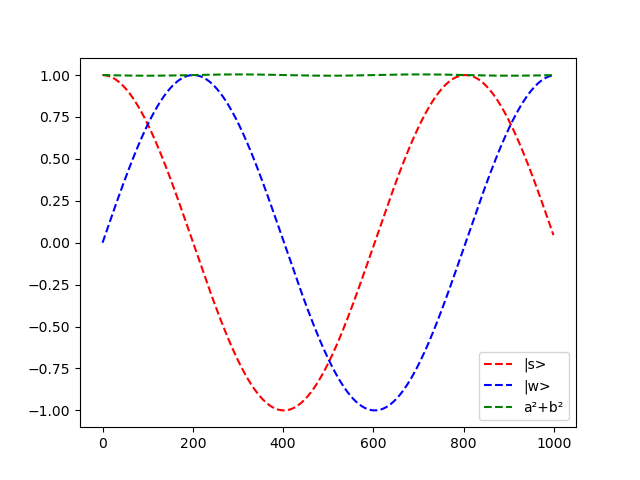
\includegraphics[scale=0.6]{Grover/grover_n16_1000.png}
  \caption{Evolution des amplitudes pour n=16, sur 1000 itérations}
  \label{fig:univerise}
\end{figure}

\subsection{Implémentation}

\subsubsection*{Simulation sur un ordinateur classique}

% \begin{lstlisting}[language=Python]
% import numpy as np
% import math
% import random

% N = 2**8
% n_opti = (math.pi/4)*math.sqrt(N)
% nb_iter = math.floor(n_opti)
% w = np.zeros((N, 1))
% w[random.randint(-1, N)] = np.imag(0 + 1j)
% s = np.ones((N, 1)) / math.sqrt(N)
% u_w = np.identity(N) - 2 * w * np.transpose(w)
% u_s = 2 * s * np.transpose(s) - np.identity(N)
% g = np.dot(u_s, u_w)
% x = s
% for i in range(0, nb_iter):
%     x = np.dot(g, x)
% \end{lstlisting}

\begin{algorithm}[H]
  \SetAlgoLined
  \KwData{
    $w$ vector of size $2^n$ of $0$ with target index to 1;
  }

  \KwOut{
    $x$ vector of amplitudes (largest amplitude corresponding to wanted index)
  }

  \Begin{
    $s$ vector of size $2^n$ of $\frac{1}{\sqrt{2^n}}$
    $N \longleftarrow 2^n$\;
    $N_{iter} \longleftarrow floor(\frac{\pi}{4} \sqrt{N})$\;
    \tcc{Compute grover operator}
    $U_w \longleftarrow I_N - 2 w \cdot w^T$\;
    $U_s \longleftarrow 2 s \cdot s^T - I_N$\;
    $g \longleftarrow U_s \cdot U_w$\;
    $x \longleftarrow s$ \;
    \tcc{Apply grover operator $N_{iter}$ times}
    \For(){$i = 0$ \KwTo $N_{iter}$}{
      $x \longleftarrow g \cdot x $\;
    }
  }
\end{algorithm}

% \subsubsection*{Algorithme quantique}

% \begin{lstlisting}[language=Python]
% import numpy as np
% import math
% import random
% from qiskit import QuantumRegister, ClassicalRegister, QuantumCircuit

% var_qubits = QuantumRegister(4, name='v')
% clause_qubits = QuantumRegister(4, name='c')
% output_qubits = QuantumRegister(1, name='out')
% cbits = ClassicalRegister(4, name='cbits')
% qc = QuantumCircuit(var_qubits, clause_qubits, output_qubits, cbits)
% qc.initialize([1, -1]/np.sqrt(2), output_qubits)
% qc.h(var_qubits)
% qc.barrier()

% \end{lstlisting}

\end{appendix}
% \chapter{Quantum Fourier Transform}


\clearpage
\addcontentsline{toc}{chapter}{Bibliographie}
\bibliographystyle{ieeetr}
\bibliography{biblio}

\clearpage
\thispagestyle{empty}

\vspace*{\fill}
\noindent\rule[2pt]{\textwidth}{0.5pt}\\
{\textbf{Résumé ---}}
Ce rapport bibliographique présente les différents éléments de base necessaires à la compréhension de l'informatique quantique. On y présente en premier les concepts fondateurs de l'informatique quantique: le qubit, les mécanismes d'évolution des systèmes quantiques et enfin la mesure projective. On y montre ensuite trois algorithmes fondateurs en illustrant les problèmes résolus et leur fonctionnement.

L'apport de l'informatique quantique est montré en insistant sur la capacité à paralléliser les opérations sur une certaine catégorie de problèmes.

{\textbf{Mots clés :}}
Informatique quantique, qubit, mesure projective, Deutsch-Jozsa, Grover, Shor, parralélisation.
\\
\noindent\rule[2pt]{\textwidth}{0.5pt}


\vspace*{\fill}
\noindent\rule[2pt]{\textwidth}{0.5pt}\\
{\textbf{Abstract ---}}
This bibliographic report presents the fundamental aspects of quantum computing. We firstly show 3 concepts required to understand quantum computing: the notion of qubit, the mecanisms of evolution of quantum systems and the projective measurement of qubits. We then show three major quantum algorithms (Deustch-Jozsa, Grover and Shor), explaining the problems they solve and how they work.

With this report, we understand how quantum computing improves the solving of a certain category of problems, via parallelism. 

{\textbf{Keywords :}}
Quantum computing, qubit, projective measurement, Deutsch-Jozsa, Grover, Shor, parallelism.
\\
\noindent\rule[2pt]{\textwidth}{0.5pt}

\begin{center}
  Polytech Angers\\
  62, avenue Notre Dame du Lac\\
  49000 Angers
\end{center}
\vspace*{\fill}

\end{document}